% SVN info for this file
\svnidlong
{$HeadURL$}
{$LastChangedDate$}
{$LastChangedRevision$}
{$LastChangedBy$}

\chapter{Geometria proiettiva}
\labelChapter{geoproiettiva}

\begin{introduction}
	‘‘La Geometria proiettiva è tutta la Geometria.''
	\begin{flushright}
		\textsc{Arthur Cayley,} cercando di vendere i suoi appunti di Geometria proiettiva agli ignari studenti di Geometria uno.
	\end{flushright}
\end{introduction}]
\lettrine[findent=1pt, nindent=0pt]{A}{bbiamo} già trattato lo \textit{spazio proiettivo reale} e le sue caratteristiche nel \autoref{chap:azionidigruppo} e \autoref{chap:varietà}. In questo, ci dedicheremo a generalizzare il concetto per un \textit{qualsiasi} spazio vettoriale su campo $\kamp$, utilizzando gli strumenti dell'algebra lineare.\\
Parliamo dunque di \textbf{Geometria proiettiva}: come in topologia studiavamo le proprietà degli spazi topologici invarianti per omeomorfismi, lo scopo della geometria proiettiva è studiare quelle degli \textbf{spazi proiettivi} invarianti per \textbf{proiettività}.
\section{Spazi proiettivi}
\begin{define}[Spazio proiettivo.]~{}\\
Sia $\kamp$ un campo e $V$ uno spazio vettoriale di dimensione \textit{finita} su $\kamp$. Lo \textbf{spazio proiettivo}\index{spazio!proiettivo} associato a $V$ è l'insieme quoziente:
\begin{equation}
	\proj{V}=\frac{V\setminus\left\{0\right\}}{\sim}
\end{equation}
Dove $\sim$ è la relazione di equivalenza data su $V\setminus\left\{0\right\}$ definita dall'azione del gruppo moltiplicativo $\kamp\setminus\left\{0\right\}$:
\begin{equation}
	\forall v,\ w\in V\setminus\left\{0\right\}\ v\sim w \iff \exists \lambda\in\kamp\setminus\left\{0\right\}\ \colon v=\lambda w
\end{equation}
Lo spazio proiettivo $\proj{V}$ si dice anche il \textbf{proiettivizzato}\seeonlyindex{proiettivizzato}{spazio!proiettivo} di $V$.
\end{define}
\begin{demonstration}
Dimostriamo che è una relazione di equivalenza:
\begin{itemize}
\item \textsc{Riflessiva}: $v\sim v?$ Basta porre $\lambda=1$, in quanto $x=1\cdot x$.
\item \textsc{Simmetrica}: Per ipotesi $y=\lambda x$, allora $x=\frac{1}{\lambda} y$ ($\frac{1}{\lambda}\in \kamp\setminus\left\{0\right\}$).

\item \textsc{Transitiva}: Poiché $y=\lambda x,\ z=\mu y$, segue $z=\mu \left(\lambda x\right)=\left(\mu\lambda\right)x$ e $\mu\lambda\in \kamp\setminus\left\{0\right\}$.
\end{itemize}
\vspace{-3mm}
\end{demonstration}
\begin{define}[Dimensione di uno spazio proiettivo.]~{}\\
La \textbf{dimensione}\index{dimensione di uno spazio proiettivo} di $\proj{V}$ è:
\begin{equation}
	\dim\proj{V}=\dim V-1
\end{equation}
Se $V=\left\{0\right\}$, allora $\proj{V}=\emptyset$ e si pone $\dim\emptyset\coloneqq -1$.
\end{define}
\begin{define}[Proiezione al quoziente e classe.]~{}\\
Si denota con $\funz{\pi}{V\setminus\left\{0\right\}}{\proj{V}}$ la \textbf{proiezione al quoziente}\index{proiezione!al quoziente} e con $\left[v\right]\in\proj{V}$ la \textbf{classe}\index{classe!dello spazio proiettivo} di $v\in V\setminus\left\{0\right\}$.
\end{define}
\begin{observe}
	Si ha una corrispondenza biunivoca:
	\begin{equation}
		\begin{array}{c}
			\proj{V}\leftrightarrow\left\{\text{sottospazi vettoriali }1\text{-dimensionali di }V\right\}\\
			\left[v\right]\leftrightarrow\lin{v}
		\end{array}
	\end{equation}
In altre parole, possiamo pensare a $\proj{V}$ come l'insieme delle \textbf{rette vettoriali} in $V$.
\end{observe}
\begin{define}[Altre nomenclature proiettive.]~{}\\
	\begin{itemize}
		\item Se $\dim V=1$, allora $\proj{V}$ è un \textbf{punto}\index{punto!proiettivo} e $\dim\proj{V}=0$.
		\item Se $\dim \proj{V}=1$, si parla di \textbf{retta proiettiva}\index{retta!proiettiva}.
		\item Se $\dim \proj{V}=2$, si parla di \textbf{piano proiettivo}\index{piano!proiettivo}.
		\item Se $\kamp=\realset$ o $\kamp=\complexset$, si parla rispettivamente di \textbf{spazio proiettivo reale}\index{spazio!proiettivo!reale} o di \textbf{spazio proiettivo complesso}\index{spazio!proiettivo!complesso}.
	\end{itemize}
\vspace{-3mm}
\end{define}
Gli esempi più frequenti di spazi proiettivi si ottengono considerando $V=\kamp^{n+1}$.
\begin{define}[Spazio proiettivo numerico.]~{}\\
	Lo \textbf{spazio proiettivo numerico}\index{spazio!proiettivo!numerico} o \textbf{spazio proiettivo standard}\seeonlyindex{spazio!proiettivo!standard}{spazio!proiettivo!numerico} è lo spazio proiettivo su $\kamp^{n+1}$:
\begin{equation}
	\proj{\ }=\proj[n]{\kamp}=\proj{\kamp^{n+1}}
\end{equation}
Essi sono spazi di dimensione $\dim\proj[n]{\ }=n$.
\end{define}
\section{Sottospazi proiettivi}
Sia $W\subseteq V$ un sottospazio vettoriale. Allora $W\setminus\left\{0\right\}\subseteq V\setminus\left\{0\right\}$ è chiuso rispetto alla relazione di equivalenza $\sim$ precedentemente definita e $\proj{W}$ è naturalmente un sottoinsieme di $\proj{V}$.
\begin{define}[Sottospazio proiettivo.]~{}\\
	Se $W\subseteq V$ è un sottospazio vettoriale, allora $\proj{W}$ è detto \textbf{sottospazio proiettivo}\index{sottospazio!proiettivo}:
	\begin{equation*}
		\begin{array}{rl}
			\proj{W}&=\pi\left(W\setminus\left\{0\right\}\right)=\left\{\left[w\right]\in\proj{V}\mid w\in W\right\}\\
			&=\left\{\text{sottospazi vettoriale }1\text{-dimensione di }V\text{ contenuti in }W\right\}
		\end{array}
	\end{equation*}
La dimensione del sottospazio proiettivo è $\dim\proj{W}=\dim W-1$.
\end{define}
	\begin{itemize}
	\item Se $W=\left\{0\right\}$, allora $\proj{W}=\emptyset$.
	\item Se $\dim W=1$, allora $\proj{W}$ è un punto, che indichiamo con $\left[w\right]$ per un $w\in W$.
	\item Se $\dim W=2$ ($\dim\proj{W}=1$), allora $\proj{W}$ è \textbf{retta proiettiva} in $\proj{V}$.
	\item Se $\dim W=3$ ($\dim\proj{W}=2$), allora $\proj{W}$ è \textbf{piano proiettivo} in $\proj{V}$.
	\item Se $\dim\proj{W}=\dim \proj{V}-1$, allora $\proj{W}$ è \textbf{iperpiano (proiettivo)}\index{iperpiano!proiettivo} in $\proj{V}$.
\end{itemize}
\begin{define}[Codimensione.]~{}\\
Si definisce la \textbf{codimensione}\index{codimensione} di $\proj{W}$ sottospazio proiettivo come:
\begin{equation}
	\codim\proj{W}=\dim\proj{V}-\dim\proj{W}
\end{equation}
\vspace{-6mm}
\end{define}
\begin{example}
	Gli iperpiani sono sottospazi di codimensione $1$.
\end{example}
\section{Coordinate omogenee e sistemi di riferimento proiettivo}
Consideriamo $\proj[n]{\kamp}=\proj{\kamp^{n+1}}$. Se $v=\left(x_0,\ \ldots,\ x_n\right)\in\kamp^{n+1}\setminus\left\{0\right\}$, denotiamo la corrispettiva classe in questa forma:
\begin{equation}
\left[v\right]=\left(x_0\colon \ldots\colon x_n\right)\in\proj[n]{\kamp},\ x_i\in\kamp
\end{equation}
\begin{observes}~{}
	\begin{enumerate}
		\item Le $x_i$ non possono mai essere tutte nulle, dato che $v\neq 0$.
		\item Due classi sono uguali se le componenti sono tutte in proporzione per uno scalare $\lambda\in\kamp$.\footnote{La notazione con i $\colon$ viene utilizzata per mettere in evidenza che la relazione fra classi e vettori è di proporzione.}
		\begin{equation*}
			\begin{array}{ccc}
			\left(x_0:\ldots:x_n\right)=\left(y_0:\ldots:y_n\right)&\iff&\left(x_0,\ \ldots,\ x_n\right)\sim\left(y_0,\ \ldots,\ y_n\right)\\&\iff& \exists \lambda\in\kamp\setminus\left\{0\right\}\ \colon y_0=\lambda x_0,\ \ldots,\ y_n=\lambda x_n
			\end{array}
		\end{equation*}
	\end{enumerate}
\end{observes}
\begin{examples}
	In $\proj[2]{\realset}$:
	\begin{gather*}
		\left(1\colon1\colon2\right) = \left(-2\colon-2\colon-4\right)\\
		\left(1\colon0\colon2\right) = \left(\frac{1}{3}\colon0\colon\frac{1}{3}\right)
	\end{gather*}
\vspace{-6mm}
\end{examples}
\begin{define}[Riferimento proiettivo e coordinate omogenee.]~{}\\
	Sia $\basis=\left\{e_0,\ \ldots,\ e_n\right\}$ una base di $V$, con $\dim V=n+1$. Se $v\in V\setminus\left\{0\right\}$, si ha:
	\begin{equation*}
		v=x_0e_0+\ldots+x_ee_n,\ \text{con}\ x_i\in\kamp
	\end{equation*}
Diciamo che $\left(x_0\colon\ldots\colon x_n\right)$ sono le \textbf{coordinate omogenee}\index{coordinate omogenee} di $\left[v\right]\in\proj{V}$ definite dalla base $\basis$ e scriviamo:
\begin{equation}
	\left[v\right]=\left(x_0\colon\ldots\colon x_n\right)
\end{equation}
La base $\basis$ definisce su $\proj{V}$ un \textbf{sistema di riferimento proiettivo}, cioè ad ogni punto vengono assegnate delle coordinate omogenee.
\end{define}
\begin{observes}~{}
		\begin{itemize}
		\item Le coordinate omogenee non possono \textit{mai} essere \textit{tutte nulle}.
		\item Le coordinate omogenee sono definite \textit{solo a meno di multipli}.
		\item $\proj[n]{\kamp}$ ha delle coordinate omogenee ‘‘naturali'' date dalla base canonica di $\kamp^{n+1}$.
		\item Basi \textit{multiple} definiscono lo stesso riferimento proiettivo di $\proj{V}$, cioè le stesse coordinate omogenee.
	\end{itemize}
\vspace{-3mm}
\end{observes}
\begin{demonstration}
	Dimostriamo l'ultimo punto. Siano:
	\begin{equation*}
		\basis=\left\{e_0,\ \ldots,\ e_n\right\}\quad\basis'=\left\{\mu e_0,\ \ldots,\ \mu e_n\right\}
	\end{equation*}
Con $\mu\in\kamp\setminus\left\{0\right\}$. Si ha:
\begin{equation*}
	v=x_0e_0+\ldots+x_ne_n=\frac{x_0}{\mu}\left(\mu e_0\right)+\ldots + \frac{x_n}{\mu}\left(\mu e_n\right)
\end{equation*}
Passando allo spazio proiettivo:
\begin{equation*}
\underbrace{\left(x_0\colon\ldots\colon x_n\right)}_{\text{coordinate omogenee rispetto a }\basis}=\underbrace{\left(\frac{x_0}{\mu}\colon\ldots\colon \frac{x_n}{\mu}\right)}_{\text{coordinate omogenee rispetto a }\basis'}
\end{equation*}
\end{demonstration}
\begin{define}[Punti fondamentali e punto unità.]~{}\\
	Data la base $\basis$, i punti:
	\begin{equation}
		\begin{array}{l}
			P_0=\left[e_0\right]=\left(1\colon0\colon\ldots\colon0\right)\\			P_1=\left[e_1\right]=\left(0\colon1\colon\ldots\colon0\right)\\
			\ldots\\
			P_n=\left[e_n\right]=\left(0\colon0\colon\ldots\colon1\right)\\
		\end{array}
	\end{equation}
Sono detti \textbf{punti fondamentali}\index{punto!fondamentale} o \textbf{punti coordinati}\seeonlyindex{punto!coordinato}{punto!fondamentale}, mentre il punto:
\begin{equation*}
	U=\left[e_0+e_1+\ldots+e_n\right]=\left(1\colon1\colon\ldots\colon1\right)
\end{equation*}
È detto \textbf{punto unità}\index{punto!unità}.
\end{define}
\subsubsection{Descrizione dei sottospazi proiettivi in coordinate}
Siano $\left(x_0\colon\ldots\colon x_n\right)$ coordinate omogenee su $\proj{V}$, indotte da una base $\basis$, e consideriamo l'equazione lineare omogenea:
\begin{equation*}
	\textcolor{green}{\circled{\ast}}\quad a_0x_0+a_1x_1+\ldots+a_nx_n=0
\end{equation*}
Con $a_i\in\kamp$ non tutti nulli.
\begin{itemize}
	\item In $V$ l'equazione omogenea rappresenta un \textit{iperpiano vettoriale} $H$.
	\item I punti $P=\left[v\right]\in\proj{V}$, le cui coordinate soddisfano l'equazioni, sono quelli tali per cui $v\in H$, cioè sono tutti e soli i punti dell'iperpiano proiettivo $\proj{H}\subseteq\proj{V}$. L'equazione lineare $\textcolor{green}{\circled{\ast}}$ è l'\textbf{equazione (cartesiana) dell'iperpiano proiettivo} $\proj{H}$.
\end{itemize}
\begin{define}[Iperpiano coordinato.]~{}\\
	Gli iperpiani di equazione cartesiana $x_i=0$, cioè tutti i punti la cui $i$-esima coordinata omogenea è nulla, si dicono $i$\textbf{-esimi iperpiani coordinati}\index{iperpiano!proiettivo!coordinato}.
\end{define}
\begin{example}\item
	In $\proj[1]{\kamp}$, cioè una \textit{retta proiettiva} ($\dim \proj[1]{\kamp}=1$), i sottospazi proiettivi sono:
	\begin{itemize}
		\item $\emptyset$.
		\item I punti, che in questo caso sono gli iperpiani.
		\item Tutto $\proj[1]{\kamp}$.
	\end{itemize}
Il punto $\left(a\colon b\right)$ ha equazione cartesiana:
\begin{equation}
	bx_0-ax_1=0
\end{equation}
Ovvero l'equazione della retta in $\kamp^2$ generata dal vettore $\left(a,\ b\right)$, ottenuta pertanto dal determinante $\left| \begin{array}{cc}
	a & b \\
	x_0 & x_1
\end{array} \right|=0$.
\end{example}
\begin{attention}
	In $\proj{V}$ un sottospazio proiettivo di \textit{dimensione zero} è un singolo punto $\left[v\right]=\proj{\lin{v}}$.
\end{attention}
Più in generale: fissata una base $\basis$ di $V$, ogni \textit{sottospazio vettoriale} $W$ di $V$ può essere visto, in \textit{coordinate} rispetto alla base, come l'\textit{insieme delle soluzioni} di un \textit{sistema lineare omogeneo}.
\begin{equation*}
	Ax=O
\end{equation*}
Dove $A=\left(a_{ij}\right)$ è di dimensioni $t\times \left(n+1\right)$ a elementi in $\kamp$, mentre si ha:
\begin{gather}
	x=\left(\begin{array}{c}
		x_0 \\
		\vdots \\
		x_n
	\end{array}\right)\\
\textcolor{green}{\circled{\ast}}\begin{cases}
	a_{1,0}x_0+\ldots+a_{1,n}x_n=0\\
	\vdots\\
	a_{t,0}x_0+\ldots+a_{t,n}x_n=0\\
\end{cases}
\end{gather}
Il sistema $\textcolor{green}{\circled{\ast}}$ dà delle \textit{equazioni cartesiane} per il sottospazio proiettivo $\proj{W}$ nelle coordinate omogenee $\left(x_0\colon\ldots\colon x_n\right)$.\\
Posto dunque $t$ come il numero delle \textit{equazioni}, notiamo che:
\begin{equation*}
	\begin{array}{cc}
		\dim W=n+1-\rk A \\
\begin{array}{lll}
	\codim W &=&\rk A \\
	\shortparallel &  \\
	\dim V-\dim W &=&\dim\proj{V}-\dim\proj{W}=\codim\proj{W}
\end{array}\\
	\implies t\geq \rk\left(A\right)=\codim\proj{W}
	\end{array}
\end{equation*}
\textit{Scartando} delle equazioni possiamo sempre ricondurci ad un sistema in cui:
\begin{equation}
	t=\rk A=\codim\proj{W}
\end{equation}
\vspace{-6mm}
\begin{intuit}
	Per facilitare la visualizzazione degli spazi proiettivi possiamo pensare allo spazio $\kamp^{n+1}$ come lo \textbf{spazio affine} $\aff{\kamp^{n+1}}$ in cui sia fissato un punto $O$ come origine: in questo modo, le classi di $\proj[n]{\kamp}$ corrispondono alle \textit{rette affini passanti per} $O$ (identificate con le rette vettoriali di $\kamp^{n+1}$):
	\begin{equation*}
		\left(x_0\colon\ldots\colon x_n\right)\leftrightarrow\begin{array}{c}
			\text{retta affine di }\aff{\kamp^{n+1}}\text{ formata}\\
			 \text{dai punti }\left(tx_0,\ \ldots,\ tx_n\right)\text{ al variare di t}\in\realset
		\end{array}
	\end{equation*}
	Approfondiremo formalmente la relazione tra gli spazi affini e gli spazi proiettivi più avanti, a pag. \ref{spaziaffini}.
\end{intuit}
\begin{examples}~{}
	\begin{itemize}
		\item Il piano proiettivo $\proj[2]{\kamp}$ ha, come sottospazi \textit{non banali}, i punti e le rette.
		\begin{itemize}
			\item Una \textit{retta proiettiva} viene da un \textit{piano}, che nel riferimento \textit{affine} possiamo prendere passante per l'origine: $a_0x_0+a_1x_0+a_2x_2=0$.
			\item Un \textit{punto} servono due equazioni, in sostanza vedendolo come \textit{intersezione di due rette proiettive}; ad esempio, $\left(1\colon0\colon0\right)$ ha equazioni $x_1=x_2=0$, mentre $\left(1\colon2\colon3\right)$ ha equazioni $\begin{cases}
				x_1=2x_0\\
				x_2=3x_0
			\end{cases}$
		\end{itemize}
	\item Nel piano proiettivo reale $\proj[2]{\realset}$, le \textit{rette proiettive} vengono da \textit{piani vettoriali}, dunque nel modello affine di $\aff{\realset^3}$ essi sono piani passanti per l'\textit{origine}; utilizzando la \textit{sfera unitaria}, i cui punti antipodali sono identificati in una relazione di equivalenza, la retta proiettiva si visualizza facilmente come l'\textit{intersezione} della sfera in un \textit{cerchio massimo}; nel modello della \textit{calotta superiore}, prendiamo l'intersezione dall'equatore in su.\\
	In questo modo, la \textbf{proiezione verticale} dell'intersezione del cerchio massimo con la calotta sul disco unitario $D$ è la rappresentazione della retta proiettiva sul \textit{modello piano del disco}. Dunque, abbiamo \textit{tre tipi} di rette:\\
	\begin{minipage}{0.77\textwidth}
			\begin{enumerate}[series=proj]
			\item La \textit{retta} con equazione $z=0$, ovvero al piano $xy$ in $\realset^3$: sul modello piano corrisponde al \textbf{bordo del disco} $D$ (cioè $S^1$).
		\end{enumerate}
		\end{minipage}
	\begin{minipage}{0.32\textwidth}
		
\includegraphics[trim=0cm 0cm 0cm 0cm,clip,scale=0.50]{images/projectivelinesdisk1.pdf}
	\end{minipage}\\
	\begin{minipage}{0.77\textwidth}
	\begin{enumerate}[resume=proj]
			\item Le \textit{rette} con equazione $ax+by=0$, ovvero ai \textit{piani perpendicolari} in $\realset^3$ passanti per le rette con quell'equazione $ax+by=0$:  sul modello piano corrisponde a \textbf{diametri colleganti due punti} sul bordo.
		\end{enumerate}
	\end{minipage}
\begin{minipage}{0.32\textwidth}
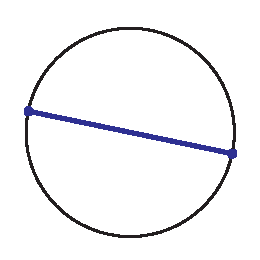
\includegraphics[trim=0cm 0cm 0cm 0cm,clip,scale=0.50]{images/projectivelinesdisk2.pdf}
\end{minipage}\\
\begin{minipage}{0.77\textwidth}
	\begin{enumerate}[resume=proj]
			\item Nel caso generale $ax+by+cz=0$, proiettando l'\textit{arco di cerchio massimo} viene un \textbf{arco di ellisse} in $D$.
		\end{enumerate}
	\end{minipage}
	\begin{minipage}{0.32\textwidth}
		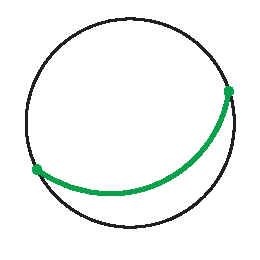
\includegraphics[trim=0cm 0cm 0cm 0cm,clip,scale=0.50]{images/projectivelinesdisk3.pdf}
	\end{minipage}
	\end{itemize}
\vspace{-3mm}
\end{examples}
\section{Operazioni con i sottospazi}
Se $W_1,\ W_2\subseteq V$ sono sottospazi vettoriali, allora $W_1\cap W_2$ è un sottospazio vettoriale e si ha che l'\textbf{intersezione}\index{sottospazio!intersezione} dei corrispettivi spazi proiettivi è ancora un sottospazio proiettivo.
\begin{equation*}
	\proj{W_1\cap W_2}=\proj{W_1}\cap\proj{W_2}
\end{equation*}
\vspace{-6mm}
\begin{observe}
	Si ha:
	\begin{equation*}
		\proj{W_1}\cap\proj{W_2}=\emptyset\iff W_1\cap W_2=\left\{0\right\}
	\end{equation*}
In tal caso diciamo che i due sottospazi sono \textbf{sghembi}\index{sottospazio!proiettivo!sghembo} o \textbf{disgiunti}\seeonlyindex{sottospazio!proiettivo!disgiunto}{sottospazio!proiettivo!sghembo}.
\end{observe}
Come per i sottospazi vettoriali, in generale l'\textbf{unione} di due sottospazi proiettivi \textit{non} è un sottospazio proiettivo.
\begin{define}[Sottospazio generato da un sottoinsieme.]~{}\\
	Sia $S\subseteq \proj{V}$ un sottoinsieme non vuoto. Il \textbf{sottospazio generato}\index{sottospazio!proiettivo!generato} da $S$, denotato con $\left<S\right>$, è l'intersezione in $\proj{V}$ di tutti i sottospazi proiettivi contenenti $S$, ed è il più piccolo sottospazio contenente $S$.
\end{define}
\begin{itemize}
	\item $\left<S\right>=S\iff S$ è un sottospazio proiettivo.
	\item Se $S=\left\{P_1,\ \ldots,\ P_m\right\}$ è finito, scriviamo $\left<P_1,\ \ldots,\ P_m\right>$ per il sottospazio generato da $P_1,\ \ldots,\ P_m$.
\end{itemize}
\begin{define}[Sottospazio somma.]~{}\\
	Dati due sottospazi proiettivi $T_1,\ T_2\subseteq \proj{V}$, cioè:
	\begin{equation*}
		T_i=\proj{W_i}\quad W_i\subseteq V,\ i=1,\ 2
	\end{equation*}
	Allora il sottospazio generato da $T_1\cup T_2$ è denotato con $T_1+T_2=\left<T_1,\ T_2\right>$ e si chiama \textbf{sottospazio somma}\index{sottospazio!somma}. In particolare, si ha:
	\begin{equation}
		\left<T_1,\ T_2\right>=\proj{W_1+W_2}
	\end{equation}
\vspace{-6mm}
\end{define}
\begin{demonstration}~{}\\
	$\includedx$ $\proj{W_1+W_2}$ è un sottospazio proiettivo che contiene, in quanto $W_1\subseteq W_1+W_2,\ W_2\subseteq W_1+W_2$ vettorialmente, sia $T_1=\proj{W_1}$ sia $T_2=\proj{W_2}$. In particolare, contiene la loro unione\footnote{Ricordiamo che non è essa un sottospazio, ma un sottoinsieme.}, dunque $\left<T_1,\ T_2\right>\left<T_1\cup T_2\right>\subseteq \proj{W_1+W_2}$.\\
	$\includesx$ Abbiamo che $T_i\subseteq \left<T_1,\ T_2\right>=\proj{U}$, con $U$ un sottospazio vettoriale di $V$. In particolare, si ha che $W_1,\ W_2\subseteq U$, da cui $W_1+W_2\subseteq U$. Passando allo spazio proiettivo:
	\begin{equation*}
		\left<T_1,\ T_2\right>=\proj{U}\subseteq \proj{W_1+W_2}
	\end{equation*}
\vspace{-6mm}
\end{demonstration}
\begin{proposition}[Formula di Grassmann proiettiva.]~{}\index{formula!di Grassmann proiettiva}\\
Siano $T_1,\ T_2$ sottospazi proiettivi di $\proj{V}$. Si ha:
	\begin{equation}
				\dim\left<T_1,\ T_2\right>+\dim\left(T_1\cap T_2\right)=\dim T_1+\dim T_2
	\end{equation}
\vspace{-6mm}
\end{proposition}
\begin{demonstration}
	Posti $T_i=\proj{W_i}$, con $W_i\subseteq V$ sottospazi vettoriali. Dalla \textit{formula di Grassmann vettoriale}:
	\begin{equation*}
		\dim\left(W_1+W_2\right)+\dim\left(W_1\cap W_2\right)=\dim W_1+\dim W_2
	\end{equation*}
Sottraendo $1$ a tutte le dimensioni, otteniamo le dimensioni dei corrispettivi spazi proiettivi e dunque la formula proiettiva.
\end{demonstration}
\begin{corollary}[Condizioni sulla dimensione dell'intersezione.]~{}\\
	Siano $T_1,\ T_2$ sottospazi proiettivi di $\proj{V}$ con $\dim\proj{V}=n$. Allora:
	\begin{equation}
		\dim \left(T_1\cap T_2\right)\geq \dim T_1+\dim T_2-n
	\end{equation}
In particolare $T_1\cap T_2\neq \emptyset$ se $\dim T_1+\dim T_2\geq n$.
\end{corollary}
\begin{demonstration}
	\begin{equation*}
		\dim\left(T_1\cap T_2\right)=\dim T_1+\dim T_2-\dim\left<T_1,\ T_2\right>\geq \dim T_1+\dim T_2-n
	\end{equation*}
Chiaramente, se $\dim T_1+\dim T_2\geq n$, allora $\dim \left(T_1\cap T_2\right)\geq 0$ e dunque $T_1\cap T_2\neq \emptyset$.
\end{demonstration}
\begin{example}
	Nel piano proiettivo, due rette sono \textit{sempre incidenti}. Infatti, le rette hanno dimensione $1$, mentre $\dim\proj[2]{\kamp}=2$, dunque vale $1+1\leq 2$, pertanto due rette si incontrano sempre.
\end{example}
\begin{observe}
	Se consideriamo l'insieme \textit{finito di punti}, possiamo considerare lo spazio $S$ \textit{generato} da $P_1,\ \ldots,\ P_m$, cioè $S=\left<P_1,\ \ldots,\ P_m\right>$; inoltre, si ha:
	\begin{equation*}
		\dim S\leq m-1
	\end{equation*}
	Infatti, se $P_i=\left[v_i\right]$ con $v_i\in V$, allora:
	\begin{equation*}
		S=\underbrace{\proj{\lin{v_1,\ \ldots,\ v_m}}}_{\dim \mathcal{L} \leq m}
	\end{equation*}
\vspace{-6mm}
\end{observe}
\section{Punti linearmente indipendenti e in posizione generale}
\begin{define}[Punti linearmente indipendenti.]~{}\\
	Siano $P_1,\ \ldots, P_m\in\proj{V}$. Diciamo che i punti $P_1,\ \ldots,\ P_m$ sono \textbf{linearmente indipendenti}\index{linearmente indipendenti} se, scelti $v_1,\ \ldots,\ v_m\in V\setminus\left\{0\right\}$ tali che $P_i=\left[v_i\right]\ \forall i$, i vettori $v_1,\ \ldots,\ v_m$ sono \textit{linearmente indipendenti} in $V$.\\
	Se così non è, diciamo che $P_1,\ \ldots, P_m$ sono linearmente dipendenti.
\end{define}
\begin{observes}~{}
	\begin{itemize}
		\item La definizione è \textit{ben posta}. Dati $\lambda_1,\ \ldots,\ \lambda_m\in\kamp\setminus\left\{0\right\}$, si ha che:
		\begin{equation*}
			v_1,\ \ldots,\ v_m\text{ sono indipendenti}\iff\lambda_1 v_1,\ \ldots,\ \lambda_m v_m\text{ sono indipendenti.}
		\end{equation*}
		\item Se $\dim \proj{V}=n$, $\proj{V}$ contiene al più $n+1$ punti indipendenti.
		\item $P_1,\ \ldots,\ P_m$ sono indipendenti se e solo se $\dim\left<P_1,\ \ldots,\ P_m\right>=m-1$.
	\end{itemize}
\end{observes}
\begin{examples}~{}
	\begin{itemize}
		\item \textit{Due} punti $P,\ Q$ sono indipendenti se e solo se $P\neq Q$. Infatti, se $P=\left[v\right]$ e $Q=\left[w\right]$, allora:
		\begin{equation*}
			P\text{ e }Q\text{ sono indipendenti}\iff v\text{ e }w\text{ sono indipendenti}\iff v\nsim w\iff P\neq Q
		\end{equation*}
		In tal caso $\left<P,\ Q\right>$ è l'unico \textit{retta} contenente $P$ e $Q$, che indicheremo anche con $\overline{PQ}$.
		\item \textit{Tre} punti $P_1,\ P_2,\ P_3$ sono indipendenti se e solo se sono \textit{distinti} e \textit{non} sono \textit{allineati}, cioè appartenenti alla stessa retta. In tal caso $\left<P_1,\ P_2,\ P_3\right>$ è l'unico \textit{piano} contenente i tre punti.
	\end{itemize}
\vspace{-3mm}
\end{examples}
\begin{define}[Punti in posizione generale.]~{}\\
	Dati dei punti $P_1,\ \ldots,\ P_m\in\proj{V}$, diciamo che sono \textbf{in posizione generale}\index{in posizione generale}\index{posizione generale} se vale una delle due condizioni seguenti:
	\begin{itemize}
		\item $m\leq n+1$ e i punti sono \textit{linearmente indipendenti}.
		\item $m>n+1$ e ogni scelta di $n+1$ punti tra loro sono linearmente indipendenti.
	\end{itemize}
\vspace{-3mm}
\end{define}
\begin{example}~{}
		\begin{itemize}
		\item Se $n=1$, cioè $\proj{V}$ è una \textit{retta proiettiva}, allora $P_1,\ \ldots,\ P_m$ sono in posizione generale se e solo se $P_1,\ \ldots,\ P_m$ sono \textit{tutti distinti}.
		\item Se $n=2$, cioè $\proj{V}$ è una \textit{piano proiettivo}, allora $P_1,\ \ldots,\ P_m$ sono in posizione generale se e solo se $P_1,\ \ldots,\ P_m$ sono a $3$ a $3$ \textit{non} allineati.
	\end{itemize}
\vspace{-3mm}
\end{example}
\subsection{Impratichiamoci! Punti linearmente indipendenti}
\begin{exercise}\textsc{F.F.P., 2.1.}\\
	Si mostri che i punti del piano proiettivo reale:
	\begin{equation*}
		\left(\frac{1}{2}\colon 1 \colon 1\right)\quad \left(1\colon \frac{1}{3} \colon \frac{4}{3}\right)\quad \left(2\colon -1 \colon 2\right)
	\end{equation*}
Sono allineati, e si determini un'equazione della retta che li contiene.
\end{exercise}
\begin{solution}
	Per verificare che i $3$ punti sono allineati, dobbiamo verificare che i corrispondenti vettori di $\realset^3$ sono dipendenti. Riscriviamo i seguenti punti per facilitarci i calcoli:
\begin{equation*}
	\left(\frac{1}{2}\colon 1 \colon 1\right)=\left(1\colon 2 \colon 2\right)\quad \left(1\colon \frac{1}{3} \colon \frac{4}{3}\right)=\left(3\colon 1 \colon 4\right)
\end{equation*}
Verifichiamolo la dipendenza con il determinante.
	\begin{equation*}
		\det\left|\begin{array}{ccc}
			1 & 2 & 2\\
			3 & 1 & 4\\
			2 & -1 & 2
		\end{array}\right|=0
	\end{equation*}
L'equazione della retta è data dall'equazione del piano vettoriale in $\realset^3$ generate da $2$ dei $3$ vettori:
\begin{equation*}
	0=\left|\begin{array}{ccc}
		x_0 & x_1 & x_2\\
		1 & 2 & 2\\
		3 & 1 & 4
	\end{array}\right|=x_0\left(8-2\right)-x_1\left(4-6\right)+x_2\left(1-6\right)=6x_0+2x_1-5x_2
\end{equation*}
Verifichiamo che contenga anche il terzo:
\begin{equation*}
	6\cdot 2 + 2\cdot \left(-1\right) -5\cdot 2=0
\end{equation*}
\vspace{-6mm}
\end{solution}
\section{Rappresentazione parametrica di un sottospazio proiettivo}
Sia $S\subseteq\proj{V}$ un sottospazio proiettivo di dimensione $m$. Allora esistono sempre $m+1$ punti $P_0,\ \ldots,\ P_m\in S$ linearmente indipendenti che generano $S$. Infatti, se $S=\proj{W}$ con $W\subseteq V$ sottospazio vettoriale di dimensione $m+1$, possiamo scegliere una base $\left\{w_0,\ \ldots,\ w_m\right\}$ di $W$ tale per cui:
\begin{equation*}
	P_i=\left[w_i\right]\in S
\end{equation*}
Sono linearmente indipendenti (perché lo sono i vettori della base) e generano $S$.\\
Allora, tutti e soli i punti di $S$ sono della forma:
\begin{equation*}
	\left[\lambda_0 w_0+\ldots+\lambda_m w_m\right]\quad \lambda_0,\ \ldots,\ \lambda_m\in\kamp
\end{equation*}
Supponiamo ora di aver fissato una base $\left\{e_0,\ \ldots,\ e_n\right\}$ di $V$ e quindi di aver considerato il corrispondente \textit{riferimento proiettivo}. In coordinate vettoriali di $V$, un punto di $W$ è $x=\left(x_0,\ \ldots,\ x_n\right)$ se e solo se:
\begin{equation*}
	x=x_0e_0+\ldots+x_ne_n=\lambda_0 w_0+\ldots+\lambda_m w_m
\end{equation*}
Il punto $P_i$ in $V$ avrà coordinate $\left(P_{0,i},\ \ldots,\ P_{n,i}\right)\ \forall i=1,\ \ldots,\ m$, dunque il generico vettore $x$ di $W$ è espresso da:
\begin{equation}
	\begin{cases}
		x_0=\lambda_0 P_{0,0}+\lambda_1P_{0,1}+\ldots+\lambda_mP_{0,m}\\
		\vdots\\
		x_n=\lambda_0 P_{n,0}+\lambda_1P_{n,1}+\ldots+\lambda_mP_{n,m}
	\end{cases}
\end{equation}
Anche i punti di $S$ sono date da queste coordinate, dunque questa viene definita la \textbf{rappresentazione parametrica}\index{rappresentazione!parametrica} del sottospazio $S$, con $\left(\lambda_0\colon\ldots\colon\lambda_m\right)$ le coordinate omogenee di $\proj{W}$ date dalla base $\left\{w_0,\ \ldots,\ w_m\right\}$.
\begin{example}
	In $\proj[3]{\realset}$ consideriamo i punti:
	\begin{equation*}
		A=\left(1\colon 0\colon -1\colon 4\right)\quad B=\left(2\colon 3\colon 0\colon 5\right)
	\end{equation*}
Allora, la rappresentazione parametrica del sottospazio $S$ con $\left(\lambda\colon \mu\right)$ è:
\begin{equation*}
	\begin{cases}
		x_0=\lambda+2\mu\\
		x_1=3\mu\\
		x_2=-\lambda\\
		x_3=4\lambda-5\mu
	\end{cases}
\end{equation*}
\vspace{-6mm}
\end{example}
\subsection{Coordinate proiettive e punti in posizione generale}
\begin{observe}
	Sia $\proj{V}$ con un riferimento proiettivo fissato. Consideriamo i punti fondamentali $P_0,\ \ldots,\ P_n$ e il punto unità $U$.
	\begin{itemize}
		\item $P_0,\ \ldots,\ P_n,\ U$ sono $n+2$ punti.
		\item $P_0,\ \ldots,\ P_n,\ U$ sono in posizione generale: essendo $P_i=\left[e_i\right]$ con $e_0,\ \ldots,\ e_n$ base di $V$, allora $P_0,\ \ldots,\ P_n$ sono indipendenti. Se sostituiamo l'$i$-esimo punto con $U=\left[e_1+\ldots+e_n\right]$, allora:
		\begin{equation*}
			P_0,\ \ldots,\ \check{P}_i,\ \ldots,\ U
		\end{equation*}
	Sono indipendenti $\forall i=0,\ \ldots,\ n$.\footnote{Indichiamo con $\check{P}_{i}$ il punto che sostituiamo.}
	\end{itemize}
\vspace{-6mm}
\end{observe}
\begin{observe}
	Sia $\basis=\left\{e_0,\ \ldots,\ e_n\right\}$ una base che induce un \textit{riferimento proiettivo} su $\proj{V}$.\\
	Per ogni $i$ sia $\lambda_i\in\kamp\setminus\left\{0\right\}$ e consideriamo $v_i=\lambda_i e_i$. Allora $\basis'=\left\{v_0,\ \ldots,\ v_n\right\}$ è ancora una base e i \textit{punti fondamentali} del riferimento indotto da $\basis'$ sono \textit{gli stessi} del riferimento indotto da $\basis$. Infatti:
	\begin{equation*}
		\left[e_i\right]=\left[v_i\right]=P_i
	\end{equation*}
	Però i due riferimenti sono \textbf{diversi}; dato $v$ espresso nella base $\basis$:
	\begin{equation*}
		v=x_0e_0+\ldots+x_ne_n
	\end{equation*}
	La sua classe in $\proj{V}$, rispetto a $\basis$, è:
	\begin{equation*}
		\left[v\right]=\left(x_0\colon\ldots\colon x_n\right)
	\end{equation*}
	Possiamo partire dall'espressione di $v$ nella base $\basis$ a quella nella base $\basis'$, moltiplicando e dividendo ogni $e_i$ per il corrispettivo $\lambda_i$:
	\begin{equation*}
		v=\frac{x_0}{\lambda_0}\left(\lambda_0e_0\right)+\ldots+\frac{x_n}{\lambda_n}\left(\lambda_ne_n\right)=\frac{x_0}{\lambda_0}v_0+\ldots+\frac{x_n}{\lambda_n}v_n
	\end{equation*}
	Passiamo dunque alla base $\basis'$ alla classe in $\proj{\kamp}$:
	\begin{equation*}
		\left[v\right]=\left(\frac{x_0}{\lambda_0}\colon\ldots\colon\right)
	\end{equation*}
	Notiamo che effettivamente il punto $\left[v\right]$ non cambia, ma i riferimenti \textit{non} sono multipli e quindi sono diversi!
	\begin{itemize}
		\item \textit{Conoscere} i punti fondamentali \textit{non basta} a determinare la base $\basis$.
		\item Riferimenti proiettivi \textit{diversi} possono avere gli \textit{stessi} punti fondamentali.
	\end{itemize}
\end{observe}
\begin{observe}\label{puntigeneraleindipendentiosserva}
	Supponiamo di avere $n+2$ punti $P_0,\ \ldots,\ P_{n+1}$ in $\proj{V}$, cioè $\forall i=0,\ \ldots,\ n+1\ \exists v_i\in V\ \colon P_i=\left[v_i\right]$. Allora:
	\begin{gather*}
		P_0,\ \ldots,\ P_{n+1}\text{ sono in posizione generale}\iff v_0,\ \ldots,\ v_n\text{ sono indipendenti e}\\
		v_{n+1}=a_0v_0+\ldots+a_nv_n\text{ con }a_i\neq 0\ \forall i=0,\ \ldots,\ n
	\end{gather*}
Infatti, se $v_0,\ \ldots,\ v_n$ è una base (in quanto sono indipendenti), $v_0,\ \ldots,\ \check{v_i},\ \ldots,\ v_n,\ v_{n+1}$ sono indipendenti se e solo se $a_i\neq 0$.
\end{observe}
\begin{theorema}[Esistenza di una base dati $n+2$ punti in posizione generale.]~{}\label{puntiposizionegeneraleesistenzabase}\\
	Sia $\proj{V}$ di dimensione $n$. Dati $n+2$ punti $P_0,\ \ldots,\ P_{n+1}$ in \textit{posizione generale}, esiste una base $\basis=\left\{e_0,\ \ldots,\ e_n\right\}$ di $V$ tale che:
	\begin{equation}
		P_0=\left[e_0\right],\ \ldots,\ P_n=\left[e_n\right],\ P_{n+1}=\left[e_0+\ldots+e_n\right]
	\end{equation}
Inoltre, se $\basis'=\left\{f_0,\ \ldots,\ f_n\right\}$ è un'altra base di $V$ che soddisfa la condizione sopra, allora $\basis$ è proporzionale a $\basis$, cioè $\exists\lambda\in\kamp\setminus\left\{0\right\}\ \colon f_i=\lambda e_i\ \forall i=0,\ \ldots,\ n$.
\end{theorema}
\begin{demonstration}
	Sia $P_i=\left[v_i\right]$ al variare di $i=0,\ \ldots,\ n+1$. I punti $P_0,\ \ldots,\ P_n$ sono indipendenti\footnote{Perchè se $N+2$ punti sono in posizione generale, presi $n+1$ punti fra di loro sono indipendenti.}, dunque per definizione $v_0,\ \ldots,\ v_n$ è una base di $V$. Definiamo:
	\begin{equation*}
		v_{n+1}=\lambda_0v_0+\ldots+\lambda_nv_n\quad \lambda_i\in\kamp
	\end{equation*}
	Ma allora, per l'osservazione precedente, $\lambda_i\neq 0\ \forall i$ perché i punti sono in posizione generale.\\
	Consideriamo $_0=\lambda_0v_0,\ e_1=\lambda_1v_1,\ \ldots,\ e_n=\lambda_nv_n$. Si ha che $\basis=\left\{e_0,\ \ldots,\ e_n\right\}$ è una base di $V$ perché $\lambda_i\neq 0$\ $\forall i$. Segue che:
	\begin{gather*}
		\left[e_i\right]=\left[v_i\right]=P_i\ \forall i=0,\ \ldots,\ n\\
		\left[e_0+\ldots+e_n\right]=\left[\lambda_0v_0+\ldots+\lambda_nv_n\right]=\left[v_{n+1}\right]=P_{n+1}
	\end{gather*}
Adesso, sia $\basis')\left\{f_0,\ \ldots,\ f_n\right\}$ come da ipotesi. Allora $\left[f_i\right]=P_i=\left[e_n\right]\ \forall i=0,\ \ldots,\ n$, cioè $\exists \mu_i\in\kamp\setminus\left\{0\right\}\ \colon f_i=\mu_i e_i\ \forall i=0,\ \ldots, n$. Inoltre, soddisfa anche $\left[f_0+\ldots+f_n\right]=P_{n+1}$, pertanto:
\begin{equation*}
	\left[f_0+\ldots+f_n\right]=\left[e_0+\ldots+e_n\right]
\end{equation*}
In altre parole, $\exists \mu\in\kamp\setminus\left\{0\right\}$ tale che:
\begin{equation*}
	\begin{array}{ccc}
		f_0+\ldots+f_n&=&\mu\left(e_0+\ldots+e_n\right)\\
		\shortparallel&&\\
		\mu_0e_0+\ldots+\mu_ne_n&&
	\end{array}
\end{equation*}
$e_0,\ \ldots,\ e_n$ è una base: per l'unicità della scrittura deve essere $\mu=\mu_0=\ldots=\mu_n$, cioè $f_i=\mu e_i\ \forall i=0,\ \ldots,\ n$.
\end{demonstration}
\section{Trasformazioni proiettive}
\begin{define}[Trasformazione proiettiva e proiettività.]~{}\\
	Un'applicazione $\funz{f}{\proj{V}}{\proj{V'}}$ tra spazi proiettivi si dice \textbf{trasformazione proiettiva}\index{trasformazione!proiettiva} o \textbf{isomorfismo proiettivo}\seeonlyindex{isomorfismo!proiettivo}{trasformazione!proiettiva} se $\exists \funz{\phi}{V}{V'}$ isomorfismo che induce un altro isomorfismo lineare:
	\begin{equation}
		\begin{tikzcd}
			\widetilde{\phi}\ \colon\\
		\end{tikzcd}
			\funztot{\ }{\proj{V}}{\proj{V'}}{\left[v\right]}{\left[\phi\left(v\right)\right]}
	\end{equation}
	Tale per cui $f=\widetilde{\phi}$.\\
	Se $V=V'$, diciamo che $f$ è una \textbf{proiettività}\index{proiettività} di $\proj{V}$.
\end{define}
\begin{demonstration}~{}
	\begin{itemize}
		\item $\widetilde{\phi}$ \textbf{è ben definita}:
		\begin{enumerate}
			\item $\phi\left(v\right)\neq 0$ perché $v\neq 0$ e $\phi$ è iniettiva, pertanto $\ker\phi=\left\{0\right\}$ e dunque l'unico vettore mappato a $0$ tramite $\phi$ è solo $0$.
			\item Se $\left[v\right]=\left[w\right]$, allora $w\sim v$, cioè $w=\lambda v$ con $\lambda\in\kamp\setminus\left\{0\right\}$; segue che per linearità di $\phi$ $\phi\left(w\right)=\lambda \left(v\right)\implies \left[\phi\left(w\right)\right]=\left[\phi\left(v\right)\right]$
		\end{enumerate}
		\item $\widetilde{\phi}$ \textbf{è iniettiva}: se $\widetilde{\phi}\left(\left[v\right]\right)=\widetilde{\phi}\left(\left[w\right]\right)$, allora
		\begin{equation*}
			\left[\phi\left(v\right)\right]=\left[\phi\left(w\right)\right]\implies\exists\lambda\in\kamp\setminus\left\{0\right\}\ \colon\phi\left(w\right)=\lambda\phi\left(v\right)=\phi\left(\lambda v\right)
		\end{equation*}
	Poiché $\phi$ è iniettiva, segue che $w=\lambda v$ e dunque $\left[v\right]=\left[w\right]$.
		\item $\widetilde{\phi}$ \textbf{è suriettiva}: infatti, se $\left[w\right]\in\proj{V'}$, essendo $\phi$ suriettiva esiste un vettore $v$ tale che $w=\phi\left(v\right)$. Segue che $\left[w\right]=\left[\phi\left(v\right)\right]=\phi\left(\left[v\right]\right)$.
	\end{itemize}
\vspace{-3mm}
\end{demonstration}
Dato che spazi \textit{vettoriali} della \textit{stessa dimensione} sono sempre \textit{isomorfi}, due spazi \textit{proiettivi} della \textit{stessa dimensione} sono sempre \textit{isomorfi} e $\proj{V}$ è sempre isomorfo a $\proj[n]{\kamp}$, con $\dim V=n+1$.
\begin{lemming}[Uguaglianza di proiettività.]~{}\\
	Siano $\funz{\phi,\ \psi}{V}{V'}$ isomorfismi. Allora:
	\begin{equation}
		\widetilde{\phi}=\widetilde{\psi}\iff\exists\lambda\in\kamp\setminus\left\{0\right\}\ \colon\psi=\lambda\phi
	\end{equation}
\vspace{-6mm}
\end{lemming}
\begin{demonstration}~{}\\
$\impliessx$ Se $v\in\kamp\setminus\left\{0\right\}$, allora $\psi\left(v\right)=\lambda\psi\left(v\right)$. Segue:
\begin{equation*}
	\implies \widetilde{\psi}\left(\left[v\right]\right)=\left[\psi\left(v\right)\right]=\left[\psi\left(v\right)\right]=\widetilde{\psi}\left(\left[v\right]\right)
\end{equation*}
$\impliesdx$ Sia $h\coloneqq \funz{\phi^{-1}\circ \psi}{V}{V}$ automorfismo. Vogliamo mostrare che $h=\lambda Id_V$ con $\lambda\in\kamp\setminus\left\{0\right\}$. Se $v\in V\setminus\left\{0\right\}$, abbiamo:
\begin{equation*}
	\begin{array}{c}
\begin{array}{ccc}
	\widetilde{\phi}\left(\left[v\right]\right)&=&\psi\left(\left[v\right]\right)\\
	\shortparallel&&\shortparallel\\
	\left[\phi\left(v\right)\right]&&\left[\psi\left(v\right)\right]
\end{array}
\implies \lambda_v\in\kamp\setminus\left\{0\right\}\ \colon \phi\left(v\right)=\lambda_v\psi\left(v\right)
\implies h\left(v\right)=\psi^{-1}\left(\phi\left(v\right)\right)=\lambda_v v
\end{array}
\end{equation*}
Segue che $v$ è autovettore di $h\ \forall v\in V\setminus\left\{0\right\}$, in particolare ogni vettore non nullo è autovettore di $h$. Segue che $h$ è diagonalizzabile e ha un unico autovalore $\lambda$. Infatti, presi $\lambda_1$ e $\lambda_2$, si avrebbero i seguenti autovalori indipendenti:
\begin{equation*}
	v_1\in V_{\lambda_1}\setminus\left\{0\right\}\qquad v_2\in V_{\lambda_2}\setminus\left\{0\right\}
\end{equation*}
E considerato che:
\begin{equation*}
	\begin{array}{l}
		h\left(v_1\right)=\lambda_1 v_1\\
		h\left(v_2\right)=\lambda_2 v_2\\
		h\left(v_1+v_2\right)=\lambda\left(v_1+v_2\right)\\
		h\left(v_1+v_2\right)=h\left(v_1\right)+h\left(v_2\right)\\
	\end{array}
	\implies \lambda\left(v_1+v_2\right)=\lambda_1 v_1+\lambda_2 v_2
\end{equation*}
Da cui segue, in quanto $v_1,\ v_2,\ v_1+v_2\neq 0$, che $\lambda=\lambda_1=\lambda_2$ e quindi è unico.\\
Allora, $h=\lambda Id_{V}$ e pertanto $\phi=\lambda \psi$.
\end{demonstration}
\subsection{Gruppo lineare proiettivo}
\begin{observe}
	Consideriamo $\proj{V}$ e l'insieme delle proiettività $\funz{\ }{\proj{V}}{\proj{V}}$.
	\begin{itemize}
		\item La \textit{composizione} di proiettività è una \textit{proiettività} (banalmente \textit{indotta} dalla composizione delle applicazioni lineari).
		\item Poiché $Id_{\proj{V}}=\widetilde{Id_V}\implies$ L'identità $Id_{\proj{V}}$ è una \textit{proiettività}.
		\item Se $\widetilde{\phi}\! \funz{\! }{\proj{V}}{\proj{V}}$, allora $\widetilde{\phi^{-1}}=\funz{f^{-1}}{\proj{V}}{\proj{V}}$. In altre parole, l'\textit{inversa} di una proiettività è ancora una proiettività.
	\end{itemize}
L'insieme delle proiettività risulta un \textbf{gruppo} rispetto alla \textit{composizione}.
\end{observe}
\begin{define}[Gruppo lineare proiettivo.]~{}\\
Il \textbf{gruppo lineare proiettivo}\index{gruppo!lineare proiettivo} $\projgl{V}$ è il gruppo delle proiettività dello spazio vettoriale $V$ con operazione la composizione di proiettività ed elemento neutro $Id_{\proj{V}}$.
\vspace{-3mm}
\end{define}
\subsubsection{Descrizione matriciale del gruppo lineare proiettivo}
Consideriamo gli isomorfismi $\funz{\ }{\kamp^{n+1}}{\kamp^{n+1}}$: sappiamo che la matrice associata agli isomorfismi è una matrice invertibile, cioè si ha una \textit{isomorfismo di gruppi} fra l'insieme degli isomorfismi in $\kamp^{n+1}$ al \textit{gruppo generale lineare} $\gl\left(n+1,\ \kamp\right)$:
\begin{equation*}
	\left\{\text{isomorfismi}\funz{\ }{\kamp^{n+1}}{\kamp^{n+1}}\right\}\leftrightarrow\gl\left(n+1,\ \kamp\right)
\end{equation*}
E con il gruppo lineare proiettivo si può fare? Consideriamo:
\begin{equation}
	\funztot{\oldphi}{\gl\left(n+1,\ \kamp\right)}{\projgl[n+1]{\kamp}}{\phi_A}{\widetilde{\phi}_A}
\end{equation}
 $\phi$ è \textit{omomorfismo} di gruppi \textit{suriettivo}, ma non iniettivo. Infatti, il nucleo non è \textit{triviale}:
 \begin{equation*}
 	\ker \oldphi=\left\{\phi_A\mid \phi_A=Id_{\proj[n]{\kamp}}=\widetilde{Id}_{\kamp^{n+1}}\right\}=\left\{\phi_A\mid \phi=\lambda I,\ \lambda\in\kamp\setminus\left\{0\right\}\right\}=\left\{\phi_A\mid A=\lambda I,\ \lambda\in\kamp\setminus\left\{0\right\}\right\}
 \end{equation*}
Tuttavia, possiamo per il Teorema dell'isomorfismo per i gruppi considerare il seguente diagramma commutativo:
\[\begin{tikzcd}
	{\gl\left(n+1,\ \kamp\right)} & {\projgl[n+1]{\kamp}} \\
	{\frac{\gl\left(n+1,\ \kamp\right)}{\left\{\lambda I\ \mid\ \lambda\in\kamp\setminus\left\{0\right\}\right\}}}
	\arrow["{\pi}"', from=1-1, to=2-1]
	\arrow["{\exists \overline f}"', from=2-1, to=1-2, dashed]
	\arrow["{\oldphi}", from=1-1, to=1-2]
\end{tikzcd}\]
E si ha pertanto l'isomorfismo:
\begin{equation*}
	\projgl[n+1]{\kamp}\cong \frac{\gl\left(n+1,\ \kamp\right)}{\left\{\lambda I\mid\lambda\in\kamp\setminus\left\{0\right\}\right\}}=\frac{\gl\left(n+1,\ \kamp\right)}{\left\{\lambda I\right\}}
\end{equation*}
Si può anche considerare l'isomorfismo tra $\left\{\lambda I\mid\lambda\in\kamp\setminus\left\{0\right\}\right\}$ e $\kamp\setminus\left\{0\right\}$, e riscrivere l'isomorfismo trovato come:
\begin{equation*}
	\projgl[n+1]{\kamp}\cong \frac{\gl\left(n+1,\ \kamp\right)}{\kamp\setminus\left\{0\right\}}
\end{equation*}

\begin{example}
	Consideriamo la seguente proiettività della \textit{retta proiettiva} $\proj[1]{\realset}$:
	\begin{equation*}
		\funztot{f}{\proj[1]{\realset}}{\proj[1]{\realset}}{\left(x_0\colon x_1\right)}{\left(ax_0+bx_1\colon cx_0+dx_1\right)}
	\end{equation*}
	Considerato il gruppo lineare proiettivo $\proj[2]{\realset}=\frac{\gl\left(2,\ \realset\right)}{\left\{\lambda I\right\}}$, per definizione di $f$ si ha $f=\widetilde{\phi}$. In particolare, la matrice associata a $\phi$ è:
	\begin{equation*}
		A=\left(\begin{array}{cc}
			a & b\\
			c & d
		\end{array}\right)
	\end{equation*}
	E dunque possiamo scrivere l'applicazione lineare $\phi$ come:
	\begin{equation*}
		\funztot{f}{\realset^2}{\realset^2}{\left(\begin{array}{c}
				x_0 \\
				x_1
			\end{array}\right)}{A\left(\begin{array}{c}
				x_0 \\
				x_1
			\end{array}\right)}
	\end{equation*}
	E dunque $f$ si può anche scrivere come:
	\begin{equation*}
		\funztot{f}{\proj[1]{\realset}}{\proj[1]{\realset}}{\left[v\right]}{\left[Av\right]}
	\end{equation*}
	Notiamo che se la matrice associata a $\phi$ fosse $2A$, per \textit{proporzionalità} si avrebbe comunque la proiettività $f$. In modo analogo, $\lambda\in\realset\setminus\left\{0\right\}$ induce la \textit{stessa proiettività} $f$ di $A$.
	\vspace{-3mm}
\end{example}
\subsection{Altri aspetti delle trasformazioni proiettive}
\begin{observe}
	Se $f$ è una proiettività di $\proj{V}$ e $S\subseteq \proj{V}$ un sottospazio proiettivo, allora $f\left(S\right)$ è ancora un sottospazio proiettivo della stessa dimensione di $S$. Se $S=\proj{W}$ e consideriamo per definizione $f=\widetilde{\phi}$ con $\funz{\phi}{V}{V}$, allora:
	\begin{equation*}
		\forall \left[v\right]\in S\ f\left(\left[v\right]\right)=\widetilde{\phi}\left(\left[v\right]\right)=\left[\phi\left(v\right)\right],\ \phi\left(v\right)\in W
	\end{equation*}
	\begin{equation}
		f\left(S\right)=\proj{\phi\left(W\right)}
	\end{equation}
\vspace{-6mm}
\end{observe}
\begin{define}[Proiettivamente equivalenti.]~{}\\
	Due sottoinsiemi $A,\ B$ di $\proj{V}$ si dicono \textbf{proiettivamente equivalenti}\index{proiettivamente equivalenti} se $\exists f$ proiettività di $\proj{V}$ tale che:
	\begin{equation}
		B=f\left(A\right)
	\end{equation}
\vspace{-6mm}
\end{define}
\begin{example}
	Due sottospazi proiettivi di $\proj{V}$ della \textit{stessa} dimensione sono sempre \textit{proiettivamente equivalenti}.
\end{example}
\begin{theorema}[Esistenza e unicità di una proiettività dati $n+2$ punti in posizione generale.]~{}\label{puntigeneralitrasformazioni}\\
Siano $\proj{V}$ e $\proj{V'}$ di dimensione $n$. Siano:
	\begin{itemize}
		\item $P_0,\ \ldots,\ P_{n+1}\in\proj{V}$ $n+2$ punti in posizione generale.
		\item $Q_0,\ \ldots,\ Q_{n+1}\in\proj{V'}$ $n+2$ punti in posizione generale.
	\end{itemize}
Allora $\exists!\funz{f}{\proj{V}}{\proj{V'}}$ trasformazione proiettiva tale che $f\left(P_i\right)=Q_i\ \forall i=0,\ \ldots,\ n+1$.\\
In particolare: se una proiettività fissa $n+2$ punti ($f\left(P_i\right)=P_i\ \forall i=0,\ \ldots,\ n+1$) in posizione generale, allora è l'identità.
\end{theorema}
\begin{demonstration}~{}
	\begin{itemize}
		\item \textbf{Esistenza}: Siano, $\forall i$:
		\begin{itemize}
			\item $P_i=\left[v_i\right]\ v_i\in V$.
			\item $Q_i=\left[w_i\right]\ w_i\in V'$.
		\end{itemize}
	Sappiamo, dall'osservazione a pag. \ref{puntigeneraleindipendentiosserva}, che:
	\begin{itemize}
		\item $v_0,\ \ldots,\ v_n$ è base di $V$, con $v_{n+1}=\lambda_0v_0+\ldots+\lambda_n v_n$ con $\lambda_i\neq 0\ \forall i$.
		\item $w_0,\ \ldots,\ w_n$ è base di $V'$, con $w_{n+1}=\mu_0w_0+\ldots+\mu_n w_n$ con $\mu_i\neq 0\ \forall i$.
	\end{itemize}
		A meno di cambiare i rappresentanti dei punti, possiamo supporre senza perdita di generalità che $\lambda_i=\mu_i=1$. Si ha dunque:
		\begin{gather*}
			v_{n+1}=v_0+\ldots+v_n\\
			w_{n+1}=w_0+\ldots+w_n
		\end{gather*}
	Sia $\funz{\phi}{V}{V'}$ l'applicazione lineare tale per cui $\phi\left(v_i\right)=w_i\ \forall i=0,\ \ldots,\ n$. Per linearità:
	\begin{equation*}
		\phi\left(v_{n+1}\right)=\phi\left(v_0+\ldots+v_n\right)=\phi\left(v_0\right)+\ldots+\phi\left(v_n\right)=w_0+\ldots+w_n=w_{n+1}
	\end{equation*}
Poiché $\im \phi$ contiene una base per costruzione, $\phi$ è suriettiva. In particolare, essendo endomorfismo ($\dim V=\dim V'$), $\phi$ è anche \textit{isomorfismo}.\\
Allora $f\coloneqq\widetilde{\phi}\funz{\ }{\proj{V}}{\proj{V'}}$ è una \textit{trasformazione proiettiva} e:
\begin{equation*}
	f\left(P_i\right)=f\left(\left[v_i\right]\right)=\left[\phi\left(v_i\right)\right]=\left(w_i\right)=Q_i\ \forall i=0,\ \ldots,\ n+1
\end{equation*}
\item \textbf{Unicità}: sia $\funz{g}{\proj{V}}{\proj{V'}}$ un'altra trasformazione proiettiva tale che $g\left(P_i\right)=Q_i\ \forall i=0,\ \ldots,\ n+1$. Per definizione, esiste $\funz{\psi}{V}{V'}$ isomorfismo per cui $g=\widetilde{\psi}$ e:
\begin{equation*}
	\left[\psi\left(v_i\right)\right]=\left[w_i\right]\ \forall i
\end{equation*}
Si ha che $\exists a_i\in\kamp\setminus\left\{0\right\}$ tale che $\psi\left(v_i\right)=a_iw_i$. Allora:
\begin{equation*}
	\begin{array}{ccccc}
		a_{n+1}w_{n+1}&=&\psi\left(v_{n+1}\right)&=&\psi\left(v_0+\ldots+v_n\right)\\
		\shortparallel&&&&\shortparallel\\
		a_{n+1}\left(w_0+\ldots+w_n\right)&&&&\psi\left(v_0\right)+\ldots+\psi\left(v_n\right)\\
		\shortparallel&&&&\shortparallel\\
		a_{n+1}w_0+\ldots+a_{n+1}w_n&&&&a_0w_0+\ldots+a_nw_n
	\end{array}
\end{equation*}
Poiché $w_0,\ \ldots,\ w_n$ è base, la scrittura è unica. Segue che $a_0=a_1=\ldots=a_{n+1}=a$. Allora:
\begin{equation*}
	\begin{array}{l}
		\psi\left(v_i\right)=aw_i=a\phi\left(v_i\right)\\
		\implies \psi=a\phi\\
		\implies g=\widetilde{\psi}=\widetilde{\phi}=f
	\end{array}
\end{equation*}
	\end{itemize}
\vspace{-6mm}
\end{demonstration}
\begin{examples}~{}
	\begin{itemize}
		\item In una \textit{retta proiettiva} ($\dim 1$), una proiettività è determinata dalle immagini di $3$ \textit{punti distinti}, dato che è equivalente alla condizione di ‘‘\textit{punti in posizione generale}''.
		\item In un \textit{piano proiettivo} ($\dim 2$), una proiettività è determinata dalle \textit{immagini} di $4$ punti, a $3$ a $3$ \textit{non allineati}.
		\item Se $A,\ B\subseteq \proj{V}$ sono insiemi finiti, ciascuno contenente $k$ punti in posizione generale, con $k\leq n+2$, allora $A$ e $B$ sono sempre proiettivamente equivalenti.
	\end{itemize}
\vspace{-3mm}
\end{examples}
\begin{example}
	Approfondiamo l'ultimo esempio. In $\proj[2]{\kamp}$ ($\dim 2$), si prenda $A=\left\{P_1,\ P_2\right\},\ B=\left\{Q_1,\ Q_2\right\}$ con $P_1\neq P_2$, $Q_1\neq Q_2$. Ho due punti distinti sia in $A$ e $B$, dunque esiste sempre una proiettività $\funz{f}{\proj[2]{\ }}{\proj[2]{\ }}$ tale che $f\left(A\right)=B$.\\
	Se invece $A$ e $B$ contengono $3$ punti, se i $3$ punti in $A$ \textit{sono allineati} mentre i $3$ punti in $B$ \textit{non} lo sono, allora $A$ e $B$ \textit{non} sono proiettivamente equivalenti.
\end{example}
\subsection{Trasformazioni proiettive in coordinate}
Supponiamo di avere fissato dei \textit{riferimenti proiettivi} su $\proj{V}$ e $\proj{V'}$, dati da delle basi $\basis$ di $V$ e $\basis'$ di $V'$, e sia $\funz{f}{\proj{V}}{\proj{V}}$ una trasformazione proiettiva. Sappiamo che $f=\widetilde{\phi}$ con $\funz{\phi}{V}{V'}$ isomorfismo lineare.\\
Sia $A\in\gl\left(n+1,\ \kamp\right)$ la matrice associata a $\phi$ rispetto alle basi $\basis$ e $\basis'$. Abbiamo visto che $\phi$ è determinata solo a meno di multipli: chiaramente, lo stesso è vero anche per $A$.\\
Siano allora:
\begin{gather*}
	P=\left(x_0\colon\ldots\colon x_n\right)\in\proj{V}\\
	f\left(P\right)=\left(y_0\colon\ldots\colon y_n\right)\in\proj{V'}
\end{gather*}
Allora $\exists\rho\in\kamp\setminus\left\{0\right\}$ tale che $\rho y=Ax$.
\begin{observe}\textsc{Cambiamenti di coordinate.}\\
Se in $\proj{V}$ abbiamo due riferimenti proiettivi, uno dalla dalla base $\basis$, e uno dalla base $\basis'$, sia $M$ la \textit{matrice del cambiamento di base} in $V$ tale che:
\begin{equation*}
	x'=Mx
\end{equation*}
Con $x$ in coordinate rispetto alla base $\basis$ e $x'$ in coordinate rispetto alla base $\basis'$. Allora, se $P\in\proj{V}$ ha coordinate:
\begin{equation*}
	\left(x_0\colon\ldots\colon x_n\right)\text{ rispetto a }\basis\\
	\left(x_0'\colon\ldots\colon x_n'\right)\text{ rispetto a }\basis'
\end{equation*}
Esiste $\rho\in\kamp\setminus\left\{0\right\}$ tale che $\rho x'=M x$.
\end{observe}
\subsection{Punti fissi di proiettività}
\begin{define}[Punto fisso.]~{}\\
	Sia $\funz{f}{\proj{V}}{\proj{V}}$ una proiettività. Un \textbf{punto fisso}\index{punto!fisso} è un punto $P\in\proj{V}$ tale che:
	\begin{equation}
		f\left(P\right)=P
	\end{equation}
\vspace{-6mm}
\end{define}
Sia $\funz{\phi}{V}{V}$ un \textit{automorfismo} tale che $f=\widetilde{\phi}$, e sia $P=\left[v\right]$, con $v\in V\setminus\left\{0\right\}$. Allora:
\begin{equation*}
	\begin{array}{ll}
		& f\left(P\right)=\left[\phi\left(v\right)\right]=\left[v\right]\\
		\iff & \exists\lambda\in\kamp\setminus\left\{0\right\}\ \colon \phi\left(v\right)=\lambda v\\
		\iff & v\text{ è un autovettore per }\phi
	\end{array}
\end{equation*}
In particolare, $\phi$ è invertibile, dunque \textit{non} ha l'autovettore \textit{nullo}. Segue che i punti fissi di $f$ sono tutti e soli i punti $\left[v\right]$ con $v$ autovettore di $\phi$.
\begin{observes}~{}
	\begin{enumerate}
		\item Se $\kamp=\complexset$, allora ogni proiettività ha almeno un punto fisso, dato che $\phi$ ha sempre almeno un autovettore.
		\item Se $\kamp=\realset$ e $\dim\proj{V}=n$, allora $\dim V=n+1$. Il \textit{polinomio caratteristico} $C_\phi\left(t\right)\in\realset\left[t\right]$ ha grado $n+1$. Se $n$ è \textit{pari}, $\phi$ ha almeno un autovalore, dato che il polinomio caratteristico ha grado $n+1$ \textit{dispari}: infatti, o è di grado \textit{uno} (e quindi ha banalmente soluzione) oppure, in quanto si può decomporre in fattori a coefficienti reali al più di grado \textit{due}, ammetterà \textit{sempre} almeno un fattore di grado \textit{uno}.
		\item Portiamo un controesempio al caso $n$ dispari. Sia $\funztot{f}{\proj{\realset}}{\proj{\realset}}{\left(x\colon y\right)}{\left(-y\colon x\right)}$. La matrice $A$ associata a $f$ è:
		\begin{equation*}
			A=\left(\begin{array}{cc}
				0 & -1 \\
				1 & 0
			\end{array}\right)
		\end{equation*}
	Il polinomio caratteristico \textit{non} ha radici \textit{reali}:
	\begin{equation*}
		C_A\left(t\right)=\det\left(\begin{array}{cc}
			-t & -1 \\
			1 & -t
		\end{array}\right)=t^2-1
	\end{equation*}
Segue che $A$ non ha autovettori reali e pertanto $f$ \textit{non} ha punti fissi.
\item In generale, l'\textit{insieme} dei punti fissi di $\funz{f}{\proj{V}}{\proj{V}}$ è dato da:
\begin{equation*}
	\left\{\proj{V_{\lambda}}\mid\lambda\text{ autovalore di }\phi\right\}
\end{equation*}
Questo è un insieme di sottospazi proiettivi a 2 a 2 disgiunti.
 	\end{enumerate}
\end{observes}
\begin{define}[Insieme fisso.]~{}\\
	Se $S\subseteq\proj{V}$ è un sottospazio, diciamo che $S$ è \textbf{fisso} per $f$ proiettività se:
		\begin{equation}
		f\left(S\right)=S
	\end{equation}
	\vspace{-6mm}
\end{define}
\subsection{Impratichiamoci! Trasformazioni proiettive}
\begin{exercise}
	In $\proj[1]{\realset}$ determinare la proiettività $f$ tale che:
	\begin{equation*}
		f\left(2\colon 1\right)=\left(1\colon1\right)\quad f\left(1\colon 2\right)=\left(0\colon1\right)\quad
		f\left(1\colon -1\right)=\left(1\colon0\right)
	\end{equation*}
\vspace{-6mm}
\end{exercise}
\begin{solution}
Notiamo che i punti:
\begin{equation*}
	\left(2\colon 1\right)\quad\left(1\colon 2\right)\quad\left(1\colon -1\right)\text{ e }	\left(1\colon 1\right)\quad\left(0\colon 1\right)\quad\left(1\colon 0\right)
\end{equation*}
Sono distinti, dunque sono in posizione generale e la proiettività è garantita. Prendiamo la generica matrice $A=\left(\begin{array}{cc}
	a & b\\
	c & d
\end{array}\right)$ associata a $\phi$ indotta da $f$ e consideriamo $\rho y=Ax$:
\begin{equation*}
	\begin{cases}
		\rho y_0=ax_0+bx_1\\
		\rho y_1=cx_0+dx_1
	\end{cases}
\end{equation*}
Imponiamo il passaggio per $f\left(2\colon 1\right)=\left(1\colon1\right)$:
\begin{equation*}
	\begin{cases}
		\rho=1a+b\\
		\rho=2c+d
	\end{cases}\implies 2a+b=2c+d
\end{equation*}
In sostanza, \textit{eliminiamo} il parametro $\rho$ per ottenere un'equazione lineare \textit{omogenea} tra gli elementi della matrice.\\
Facciamo lo stesso con i rimanenti punti $f\left(1\colon 2\right)=\left(0\colon1\right)$ e $	f\left(1\colon -1\right)=\left(1\colon0\right)$, utilizzando rispettivamente $\mu y=Ax$ e $\alpha y=Ax$:
\begin{gather*}
	\begin{cases}
		0=a+2b\\
		\rho=c+2d
	\end{cases}\implies a+2b=0\\
	\begin{cases}
		\alpha=a-b\\
		0=c-d
	\end{cases}\implies c-d=0
\end{gather*}
Costruiamo così un sistema lineare omogeneo di $3$ equazioni in $4$ incognite $a,\ b,\ c,\ d$, con una matrice dei coefficienti di rango $3$:
\begin{equation*}
	\begin{cases}
		2a+b=2c+d\\
		a+2b=0\\
		c-d=0
	\end{cases}\implies \begin{cases}
	a=2c\\
	b=-c\\
	c=c\\
	d=c
\end{cases}\implies
A=\left(\begin{array}{cc}
	2c & -c\\
	c & c
\end{array}\right)=c\left(\begin{array}{cc}
1 & -1\\
1 & 1
\end{array}\right)
\end{equation*}
A meno di multipli, $A=\left(\begin{array}{cc}
	1 & -1\\
	1 & 1
\end{array}\right)$ è la matrice cercata. Segue dunque che la proiettività cercata è:
\begin{equation*}
	\funztot{f}{\proj[1]{\realset}}{\proj[1]{\realset}}{\left(x_0\colon x_1\right)}{\left(2x_0-x_1\colon x_0+x_1\right)}
\end{equation*}
\vspace{-3mm}
\end{solution}
\section{Geometria affine e geometria proiettiva}\label{spaziaffini}
Abbiamo già accennato all'esistenza di una relazione che intercorre fra \textit{geometria affine} e \textit{geometria proiettiva}. Diamo innanzitutto qualche richiamo dei concetti della geometria affine.
\begin{define}[Spazio affine.]~{}\\
	Sia $V$ uno spazio vettoriale di dimensione finita su un campo $\kamp$. Uno \textbf{spazio affine}\index{spazio!affine} di dimensione $n$ su $V$ (con spazio vettoriale associato $V$ di dimensione $n$ ) è un insieme $\aff{V}$ non vuoto di \textit{punti} (elementi) tale che sia data un'applicazione:
	\begin{equation*}
		\funztot{\ }{\aff{V}\times\aff{V} }{V}{\left(P,\ Q\right)}{\overrightarrow{PQ}}
	\end{equation*}
	Che alla coppia di punti $\left(P,\ Q\right)$ associa il vettore di $V$ con punto iniziale $P$ e punto finale $Q$ e tale che siano
	soddisfatti i seguenti assiomi:
	\begin{enumerate}
		\item $\forall P\in\aff{V},\ \forall v\in V$ esiste un unico punto $Q\in\aff{V}$ tale che $\overrightarrow{PQ}=v$.
		\item $\forall P,\ Q,\ R\in\aff{V}$ terna di punti di $\aff{V}$ si ha $\overrightarrow{PQ}+\overrightarrow{QR}=\overrightarrow{PR}$.
	\end{enumerate}
\end{define}
\begin{define}[Riferimento affine e coordinate affini.]~{}\\
	Un \textbf{riferimento affine}\index{riferimento!affine} $\mathcal{R} = (O,\  e_1,\  e_2,\ \ldots,\  e_n)$ sullo spazio $\aff{V}$ è assegnato fissando un punto $O\in \aff{V}$ detta \textbf{origine}\index{origine affine} ed una base $\basis = (e_1,\  e_2,\ \ldots,\  e_n)$ di $V$. Dunque, per ogni $P\in \aff{V}$ si ha la $n$-upla $(X_1,\  X_2,\ \ldots,\  X_n)$ dette \textit{coordinate affini}\index{coordinate!affini} del punto $P\in\aff{V}$ (uniche per riferimento affine fissato) tale per cui:
	\begin{equation}
		P=\overrightarrow{OV}=x_1e_1+\ldots+x_ne_n
	\end{equation}
\vspace{-6mm}			
\end{define}
Per i nostri scopi, parleremo spesso degli spazi affini di dimensione $n$ su $\kamp$.
\begin{define}[Affinità.]~{}\\
	Un'\textbf{affinità}\seeonlyindex{affinità}{trasformazione!lineare affine} o \textbf{trasformazione lineare affine}\index{trasformazione!lineare affine} di $\aff{\kamp^n}$ è un'applicazione:
	\begin{equation}
		\funz{\phi}{\aff{\kamp^n}}{\aff{\kamp^n}}
	\end{equation}
Della forma $\phi\left(x\right)=Ax+b$ con $A\in\gl\left(n,\ \kamp\right)$ un'applicazione lineare invertibile e $b$ una \textit{traslazione}.
\end{define}
\begin{define}[Sottospazio affine.]~{}\\
	Un \textbf{sottospazio affine}\index{sottospazio!affine} di $\aff{\kamp^n}$ è un \textit{traslato} di un sottospazio vettoriale $W\subseteq \kamp^n$:
	\begin{equation}
		S=W+x_0=\left\{w+x_0\mid w\in W,\ x_0\in\aff{W}\right\}
	\end{equation}
\vspace{-6mm}
\end{define}
\begin{observes}~{}
	\begin{itemize}
		\item $W$ è l'unico traslato di $S$ per l'origine ($x_0=O$) e si dice \textbf{sottospazio direttore}  di $S$\index{sottospazio!direttore}, cioè ne dà appunto la \textit{direzione}. Si definisce $\dim S\coloneqq\dim W$.
		\item Un punto in $\aff{\kamp^n}$ è un sottospazio affine di dimensione $0$ ($W=\left\{0\right\}$; dopotutto non ha particolarmente senso parlare di direzione del punto).
		\item Una \textbf{retta affine}\index{retta!affine} $r$ in $\aff{\kamp^n}$ è un sottospazio affine di $\dim 1$: $W=\lin{v}$, cioè $r$ si può individuare assegnando un punto $P\in r$ e un qualsiasi vettore $v$ \textit{parallelo} alla retta $r$.
		\item Un \textbf{piano affine}\index{piano!affine} $\pi$ in $\aff{\kamp^n}$ è un sottospazio affine di $\dim 2$: $W=\lin{v,\ w}$, cioè $\pi$ si può individuare assegnando un punto $P\in r$ e una coppia di vettori l.i. \textit{paralleli} al piano $\pi$.
		\item Un \textbf{iperpiano affine}\index{iperpiano!affine} è un sottospazio di dimensione $n+1$.
		\item Due sottospazi affini della stessa dimensione si dicono \textbf{paralleli}\index{sottospazio!affine!parallelo} se hanno lo \textit{stesso} sottospazio direttore.
	\end{itemize}
\vspace{-3mm}
\end{observes}
\begin{example}
Consideriamo $r=W+x_0$ retta affine, che ha dunque $\dim r=\dim W=1$. $W$ è la retta vettoriale in $\kamp^n$, mentre un qualunque $v\in W\setminus\left\{0\right\}$ è la \textit{direzione} della retta.
\end{example}
Un sottospazio affine $S\subseteq \kamp^n$ può essere descritti con equazioni cartesiane oppure in forma parametrica.\\
	\textbf{Equazioni cartesiane}. $S$ è visto come l'insieme delle \textit{soluzioni} del seguente sistema lineare:
	\begin{equation}
		Ax=b\qquad\left(\begin{array}{c}
			X_1\\
			\vdots\\
			X_n
		\end{array}\right)\in\aff{\kamp^{n}}
	\end{equation}
Con $b$ che descrive la traslazione dovuta a $x_0\in\aff{W}$.
In tal caso $W$ è il sottospazio vettoriale delle soluzioni del sistema lineare omogeneo associato:
\begin{equation}
	Ax=0
\end{equation}
\textbf{Forma parametrica}. Supponiamo $\dim S=\dim W=m$. Siano $v_1,\ \ldots,\ v_m\in\kamp^n$ i vettori di una base di $W$; rispetto ad una base di $\kamp^n$, e dunque rispetto ad un sistema di riferimento affine con origine $O$, essi sono espressi nelle componenti:
\begin{equation*}
	v_i=\left(V_{i,1},\ \ldots,\ V_{i,n}\right)\in\aff{\kamp^n}
\end{equation*}
Consideriamo $S=W+c$, con il punto $c=\left(C_1,\ \ldots,\ C_n\right)$ rispetto allo stesso sistema affine di prima.\\
I punti $x$ di $S$ in forma parametrica sono dati da:
\begin{equation}
	x=t_1v_1+\ldots+t_mv_m+c\quad t_1,\ \ldots,\ t_m\in\kamp
\end{equation}
Da cui otteniamo il sistema $n\times\left(m+1\right)$ seguente:
\begin{equation}
	\begin{cases}
		\begin{array}{l}
			X_1=t_1V_{1,1}+\ldots+t_mV_{m,1}+C_1\\
			\vdots\\
			X_n=t_1V_{1,n}+\ldots+t_mV_{m,n}+C_n\\			
		\end{array}
	\end{cases}
\end{equation}
\begin{example}
	La retta $r$ ($\dim W=1$) passante per $c$ con direzione $v$ è descritto parametricamente da:
\begin{equation*}
	\begin{cases}
		\begin{array}{l}
			X_1=tV_1+c_1\\
			\vdots\\
			X_n=tV_n+c_n			
		\end{array}
	\end{cases}
\end{equation*}	
\end{example}
Consideriamo ora lo \textit{spazio proiettivo numerico}:
\begin{equation*}
	\proj[n]{\ }=\proj[n]{\kamp}=\proj{\kamp^{n+1}}
\end{equation*}
E i punti in coordinate omogenee $\left(x_0\colon \ldots\colon x_n\right)$ rispetto ad un dato sistema di riferimento proiettivo.
Consideriamo il seguente sottoinsieme di $\proj[n]{\ }$:
\begin{equation}
	U_0\coloneqq \left\{P=\left(x_0\colon\ldots\colon x_n\right)\in \proj[n]{\ }\mid x_0\neq 0\right\}
\end{equation}
La condizione $x_0\neq 0$ è \textit{ben posta}; infatti, se $\lambda\in\kamp\setminus\left\{0\right\}$, allora $x_0\neq 0\iff\lambda x_0\neq 0$.\\
Consideriamo anche il suo complementare, che è l'iperpiano coordinato rispetto alla prima coordinata omogenea:
\begin{equation}
	\proj[n]{\ }\setminus=H_0=\left\{P=\left(x_0\colon\ldots\colon x_n\right)\in \proj[n]{\ }\mid x_0= 0\right\}=\left\{P=\left(0\colon\ldots\colon x_n\right)\in \proj[n]{\ }\right\}
\end{equation}
Sia $P\in U_0$: allora essendo $a_0\neq 0$ si ha $P=\left(a_0\colon\ldots\colon a_n\right)=\left(1\colon\frac{a_1}{a_0}\ldots\colon \frac{a_n}{a_0}\right)$. In particolare, $\frac{a_1}{a_0},\ \ldots,\ \frac{a_n}{a_0}$ sono univocamente determinate da $P$.
\begin{example}
 Sia $\proj[2]{\realset}=\left\{\text{rette vettoriali in }\realset^3\right\}$ con punti di componenti $\left(x_0\colon x_1\colon x_2\right)$. Allora $H_0$ è una retta proiettiva in $\proj[2]{\realset}$ e risulta:
 \begin{equation*}
 	\begin{array}{ll}
 		H_0 & =\left\{P=\left(x_0\colon x_1\colon x_2\right)\in \proj[n]{\ }\mid x_0=0\right\}=\left\{P=\left(0\colon x_1\colon x_2\right)\in \proj[n]{\ }\right\} \\
 		& =\left\{\text{rette vettoriali di }\realset^3\text{ contenute nel piano affine }x_0=0\right\}
 	\end{array}
 \end{equation*}
	Infatti, prendiamo $\aff{\realset^3}$ e consideriamo il piano $x_0=1$, parallelo al piano $x_0=0$. Se $r\subseteq \realset^3$ è una retta vettoriale che \textit{non} appartiene al piano affine $\left\{x_0=0\right\}$ ($r\nsubseteq \left\{x_0=0\right\}$), $r$ interseca il piano $x_0=1$ in un solo punto! In particolare, se $r$ ha direzione $\left(a_0,\ a_1,\ a_2\right)$, il punto nel piano $\left\{x_0=1\right\}$ avrà coordinate $\left(\frac{a_1}{a_0},\ \frac{a_2}{a_0}\right)$.
\end{example}
Possiamo identificare $U_0\subseteq\proj[n]{\ }$ con $\aff{\kamp^n}$. Consideriamo le due funzioni seguenti:\label{spaziaffinitoproiettivi}
\begin{equation}
	\funztot{j=j_0}{\aff{\kamp^n}}{U_0\subseteq \proj[n]{\ }}{\left(X_1,\ \ldots,\ X_n\right)}{\left(1\colon\ x_1\colon \ldots\colon X_n\right)}\\
	\funztot{\oldphi}{U_0\subseteq \proj[n]{\ }}{\aff{\kamp^n}}{\left(x_0\colon\ \ldots\colon X_n\right)}{\left(\frac{x_1}{x_0},\ \ldots,\ \frac{x_n}{x_0}\right)}
\end{equation}
\begin{itemize}
	\item $\oldphi$ è ben definita, dato che $x_0\neq 0$ per definizione di $U_0$.
	\item $j$ e $\oldphi$ sono l'una l'inversa dell'altra:
	% https://q.uiver.app/?q=WzAsNixbMCwwLCJcXGFmZntcXGthbXBebn0iXSxbMSwwLCJVXzAiXSxbMiwwLCJcXGFmZntcXGthbXBebn0iXSxbMCwxLCJcXGxlZnQoWF8xLFxcIFxcbGRvdHMsXFwgWF9uXFxyaWdodCkiXSxbMSwxLCJcXGxlZnQoMVxcY29sb24gWF8xXFxjb2xvbiBcXGxkb3RzXFxjb2xvbiBYX25cXHJpZ2h0KSJdLFsyLDEsIlxcbGVmdChYXzEsXFwgXFxsZG90cyxcXCBYX25cXHJpZ2h0KSJdLFswLDEsImoiXSxbMSwyLCJcXG9sZHBoaSJdLFszLDQsIiIsMCx7InN0eWxlIjp7InRhaWwiOnsibmFtZSI6Im1hcHMgdG8ifX19XSxbNCw1LCIiLDAseyJzdHlsZSI6eyJ0YWlsIjp7Im5hbWUiOiJtYXBzIHRvIn19fV1d
	\[\begin{tikzcd}
		{\aff{\kamp^n}} & {U_0} & {\aff{\kamp^n}} \\[-25pt]
		{\left(X_1,\ \ldots,\ X_n\right)} & {\left(1\colon X_1\colon \ldots\colon X_n\right)} & {\left(X_1,\ \ldots,\ X_n\right)}
		\arrow["{j}", from=1-1, to=1-2]
		\arrow["{\oldphi}", from=1-2, to=1-3]
		\arrow[from=2-1, to=2-2, maps to]
		\arrow[from=2-2, to=2-3, maps to]
	\end{tikzcd}\]
% https://q.uiver.app/?q=WzAsNixbMCwwLCJVXzAiXSxbMSwwLCJcXGFmZntcXGthbXBebn0iXSxbMiwwLCJVXzAiXSxbMCwxLCJcXGxlZnQoeF8wXFxjb2xvbiBcXGxkb3RzXFxjb2xvbiB4X25cXHJpZ2h0KSJdLFsxLDEsIlxcbGVmdChcXGZyYWN7eF8xfXt4XzB9LFxcIFxcbGRvdHMsXFwgXFxmcmFje3hfbn17eF8wfVxccmlnaHQpIl0sWzIsMSwiXFxsZWZ0KDFcXGNvbG9uXFxmcmFje3hfMX17eF8wfVxcY29sb25cXGxkb3RzXFxjb2xvblxcZnJhY3t4X259e3hfMH1cXHJpZ2h0KT1cXGxlZnQoeF8wXFxjb2xvblxcbGRvdHNcXGNvbG9uIHhfblxccmlnaHQpIl0sWzAsMSwiXFxvbGRwaGkiXSxbMSwyLCJqIl0sWzMsNCwiIiwwLHsic3R5bGUiOnsidGFpbCI6eyJuYW1lIjoibWFwcyB0byJ9fX1dLFs0LDUsIiIsMCx7InN0eWxlIjp7InRhaWwiOnsibmFtZSI6Im1hcHMgdG8ifX19XV0=
\[\begin{tikzcd}
	{U_0} & {\aff{\kamp^n}} & {U_0} \\[-25pt]
	{\left(x_0\colon \ldots\colon x_n\right)} & {\left(\frac{x_1}{x_0},\ \ldots,\ \frac{x_n}{x_0}\right)} & {\left(1\colon\frac{x_1}{x_0}\colon\ldots\colon\frac{x_n}{x_0}\right)=\left(x_0\colon\ldots\colon x_n\right)}
	\arrow["{\oldphi}", from=1-1, to=1-2]
	\arrow["{j}", from=1-2, to=1-3]
	\arrow[from=2-1, to=2-2, maps to]
	\arrow[from=2-2, to=2-3, maps to]
\end{tikzcd}\]
\end{itemize}
Si ha dunque che $j$ e $\oldphi$ sono \textit{biunivoche}. In questo modo identifichiamo $U_0\subseteq \proj[n]{\ }$ con $\aff{\kamp^n}$, mentre l'iperpiano $H_0$ corrisponde allo spazio proiettivo di dimensione $n-1$; si ha dunque:
\begin{equation}
	\proj[n]{\ }=U_0\amalg H_0=\aff{\kamp^n}\amalg \proj[n-1]{\ }
\end{equation}
La coppia $\left(U_0,\ j\right)$ è detta \textbf{carta affine}\index{carta affine} di $\proj[n]{\ }$.\\
In altre parole, $\proj[n]{\ }$ si può vedere come un'estensione o \textit{ampliamento} dello spazio affine $\kamp^n$. Diciamo allora che:
	\begin{itemize}
		\item I punti di $H_0$ sono detti \textbf{punti impropri}\seeonlyindex{punto!improprio}{punto!all'infinito} o \textbf{punti all'infinito}\index{punto!all'infinito}.
		\item $H_0$ è detto \textbf{iperpiano improprio}\seeonlyindex{iperpiano!improprio}{iperpiano!all'infinito} o \textbf{iperpiano all'infinito}\index{iperpiano!all'infinito}.
		\item I punti di $U_0=\aff{\kamp^n}$ sono detti \textbf{punti propri}\index{punto!proprio}.
	\end{itemize}
\begin{intuit}
In molti casi, possiamo liberamente parlare di $\aff{\kamp^n}$ come lo spazio vettoriale $\kamp^n$ inteso in senso \textit{geometrico} come insieme di punti con un punto qualunque come origine.
\end{intuit}
\begin{example}
	Consideriamo la retta proiettiva $\proj[1]{\kamp}$. L'iperpiano all'infinito è:
	  \begin{equation*}
	 		H_0=\left\{P=\left(x_0\colon x_1\right)\in \proj[1]{\ }\mid x_0=0\right\}=\left\{\left(0\colon 1\right)\right\}
	 \end{equation*}
 Mentre invece l'insieme dei punti propri è:
 \begin{equation*}
 	U_0=\left\{P=\left(x_0\colon x_1\right)\in \proj[1]{\ }\mid x_0\neq 0\right\}=\left\{\left(0\colon 1\right)\right\}
 \end{equation*}
In particolare, si ha la corrispondenza biunivoca $U_0\stackrel{1\colon1}{\leftrightarrow}\kamp$:
\begin{equation*}
	\left(x_0\colon x_1\right)=\left(1\colon \frac{x_1}{x_0}\right)\mapsto \frac{x_1}{x_0}\in\kamp
\end{equation*}
\begin{minipage}{0.56\textwidth}
In altre parole, si può vedere la retta proiettiva come il campo $\kamp$ con l'aggiunto di un unico punto, l'\textit{infinito} $\infty$.
\begin{equation}
	\proj[1]{\ }=\kamp\cup\left(0\colon 1\right)=\kamp\cup\left\{\infty\right\}
\end{equation}
Se $\kamp=\realset$, essendo $S^1\setminus\left\{1\text{ punto}\right\}\cong \realset$, si ha:
\begin{equation}
	\proj[1]{\realset}=\realset\cup\left\{\infty\right\}\cong S^1
\end{equation}
\end{minipage}
\begin{minipage}{0.44\textwidth}
	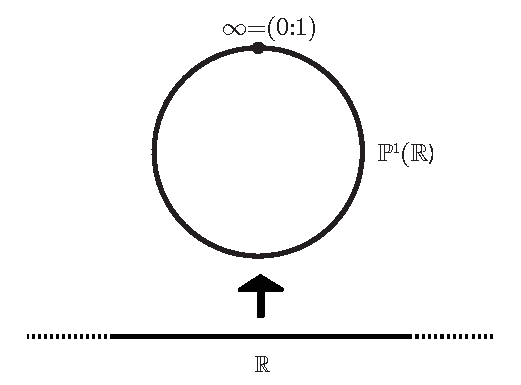
\includegraphics[trim=0cm 0cm 0cm 0cm,clip,scale=0.75]{images/projlinetocirc.pdf}
\end{minipage}
\vspace{-2mm}
\end{example}
\subsection{Chiusura proiettiva di un sottospazio affine}
\begin{define}[Chiusura proiettiva della retta affine.]~{}\\
	Sia $r\subseteq\aff{\kamp^n}$ una retta affine. La \textbf{chiusura proiettiva}\index{chiusura!proiettiva!della retta} di $r$ è il sottospazio proiettivo $\overline{r}\subseteq\proj[n]{\ }$ generato da $r\subseteq U_0\subseteq\proj[n]{\ }$.
\end{define}
\begin{proposition}[Chiusura proiettiva della retta affine.]~{}\\
	$\overline{r}$ è una \textit{retta proiettiva} e si ha:
	\begin{equation}
		\overline{r}=r\cup P_{\infty}
	\end{equation}
Dove $P_{\infty}=\overline{r}\cap H_0$ è detto \textit{punto all'infinito} o \textit{punto improprio} della retta $r$.
\end{proposition}
\begin{demonstration}
	Sia $v\in\kamp^n\setminus\left\{0\right\}$ la direzione di $r$ e $w\in r$ un punto della retta. Allora $r$ ha descrizione parametrica in $\aff{\kamp^n}$:
	\begin{equation*}
		\begin{cases}
			\begin{array}{l}
				X_1=tv_1+w_1\\
				\vdots\\
				X_n=tv_n+w_n\\			
			\end{array}
		\end{cases}\quad t\in\kamp
	\end{equation*}
Consideriamo la retta proiettiva $R\subseteq\proj[n]{\ }$ con descrizione parametrica:
\begin{equation*}
\begin{cases}
		\begin{array}{l}
			x_0=s\\
			x_1=tv_1+sw_1\\
			\vdots\\
			x_n=tv_n+sw_n\\			
		\end{array}
	\end{cases}\quad \left(s\colon t\right)\in\proj[1]{\ }
\end{equation*}
$R$ è la retta proiettiva per i punti:
\begin{equation*}
	t=0\ \colon\ \left(1\colon w_1\colon\ldots\colon w_n\right)\quad t=1\ \colon\ \left(0\colon v_1\colon\ldots\colon v_n\right)=P_\infty
\end{equation*}
Ponendo $s=1$ otteniamo:
\begin{equation*}
	\begin{cases}
		\begin{array}{l}
			x_0=1\\
			x_1=tv_1+w_1\\
			\vdots\\
			x_n=tv_n+w_n\\			
		\end{array}
	\end{cases}\quad t\in\kamp
\end{equation*}
Al variare di $t\in\kamp$, questi sono tutti e soli i punti di $j\left(r\right)\subseteq U_0\subseteq \proj[n]{\ }$. Si ha dunque che $R$ è una retta proiettiva contente $r$:
\begin{equation*}
	\begin{array}{ll}
			R&=r\cup P_{\infty}\\
			P_{\infty}&=R\cap H_0=\left\{\left(0\colon v_1\colon v_n\right)\right\}
	\end{array}
\end{equation*}
$R$ è necessariamente il più piccolo sottospazio proiettivo contenente $r$, dato che è la retta più un solo punto. Pertanto, $R=\overline{r}$.
\end{demonstration}
\begin{observes}~{}
	\begin{enumerate}
		\item Il punto improprio di $r$ è:
		\begin{equation*}
			P_{\infty}=\left(0\colon v_1\colon \ldots\colon v_n\right)
		\end{equation*}
	E corrisponde esattamente alla \textit{direzione} $v=\left(v_1,\ \ldots,\ v_n\right)$ di $r$.
	Poiché $P_\infty=\left[v\right]$ con $v$ la direzione di $r$, ne segue che l'iperpiano improprio di $\proj[n]{\kamp }$ è:
	 \begin{equation*}
		\begin{array}{ll}
			H_0 & =\proj[n-1]{\kamp}=\proj{\kamp^n}=\left\{\text{rette vettoriali in }\kamp^n\right\}=\\
			&=\left\{\text{direzioni delle rette affini in }\aff{\kamp^n}\right\}
		\end{array}
	\end{equation*}
\item Due rette affini $r_1,\ r_2\subseteq \aff{\kamp^n}$ hanno lo stesso punto improprio se e solo hanno la \textit{stessa direzione}, cioè se sono \textit{parallele}.\\
Se $r_1\neq r_2$ e $r_1$ e $r_2$ sono parallele, allora $r_1\cap r_2=\emptyset$ in $\aff{\kamp^n}$, ma $\overline{r_1}\cap \overline{r_2}={P_{\infty}}$ in $\proj[n]{\ }$. Ciò ci porta a dire che due rette parallele $r_1$ e $r_2$ si incontrano sempre all'\textit{infinito}!
\item Se $n=2$, cioè operando in $\proj[2]{\ }$, due rette distinte $r_1,\ r_2\subseteq \aff{\kamp^2}$ sono o \textit{incidenti} o \textit{parallele}, ma in $\proj[2]{\ }$ si intersecano sempre.
\item Viceversa: sia $l\subseteq \proj[n]{\ }$ una retta proiettiva. Abbiamo due casi:
\begin{itemize}
	\item $l\subseteq H_0,\ l\cap U_0= \emptyset$.
	\item $l\nsubseteq H_0\implies l+H_0=\proj[n]{\ }$.
\end{itemize}
Infatti, si ha che $l+H_0$ è un sottospazio proiettivo che contiene strettamente $H_0$, dato che $l\nsubseteq H_0$, e usando la formula di Grassmann otteniamo:
\begin{equation*}
	\dim\left(l+H_0\right)=\dim l +\dim H_0-\dim \left(l\cap H_0\right)=1+n-1+0=n=\dim \proj[n]{\ }\implies l+H_0 = \proj[n]{\ }
\end{equation*}
Sempre dalla formula di Grassmann:
\begin{equation*}
	\dim\left(l\cap H_0\right)=0\implies l\cap H_0=\left\{1 \text{punto}\right\}=\left\{Q\right\}
\end{equation*}
Cioè $l\cap U_0=l\setminus\left\{Q\right\}$. In altre parole, $l$ è una retta affine in $\aff{\kamp^n}$ con un \textit{punto improprio} $Q$ e necessariamente $l$ è la chiusura proiettiva di $l\setminus\left\{Q\right\}$.
\item Sia $n=2$, cioè operiamo in $\proj[2]{\ }$. Una retta $r\subseteq \aff{\kamp^2}$ è descritta da un'equazione lineare:
\begin{equation}
	ax+by+c=0\quad \left(a,\ b\right)\neq\left(0,\ 0\right)
\end{equation}
Con la corrispondenza biunivoca fra le coordinate $\left(x,\ y\right)$ vettoriali e $\left(X_1,\ X_2\right)$ affini. Abbiamo tuttavia anche la corrispondenza con le coordinate omogenee in $\proj[2]{\ }$, rispettivamente $\left(x\colon y\colon z\right)$ e $\left(_0\colon x_2\colon x_3\right)$.\\
Chiamiamo $\left(x\colon y\colon z\right)$ le coordinate omogenee su $\proj[2]{\ }$ con:
\begin{equation*}
	H_0=\left\{P=\left(x\colon y\colon z\right)\in \proj[2]{\ }\mid z=0\right\}=\left\{P=\left(x\colon y\colon0\right)\in \proj[2]{\ }\right\}
\end{equation*}
Allora la chiusura proiettiva $\overline{r}\subseteq \proj[2]{\ }$ di $r$ ha in $\proj[2]{\ }$ l'equazione lineare omogenea seguente:
\begin{equation}
		ax+by+cz=0
\end{equation}
Infatti, per $z=1$ si ottiene l'equazione di $r$, mentre ponendo $z=0$ (cioè il passaggio per $H_0$) troviamo il punto improprio $P_{\infty}$ di $r$:
\begin{equation*}
		\begin{cases}
		\begin{array}{l}
			z=0\\
			ax+by=0\\	
		\end{array}
	\end{cases}\quad P_{\infty}=\left(-b\colon a\colon 0\right)
\end{equation*}
La direzione della retta $ax+by+c=0$ è data dal punto improprio $P_{\infty}$ e corrisponde al vettore $\left(-b, a\colon 0\right)$.
	\end{enumerate}
\end{observes}
Generalizziamo ora il concetto di chiusura proiettiva a un generico sottospazio affine.
\begin{define}[Chiusura proiettiva di un sottospazio.]~{}\\
	Dato $S\subseteq \aff{\kamp^n}$ un sottospazio affine con $S\neq \emptyset$, la \textbf{chiusura proiettiva}\index{chiusura!proiettiva} $\overline{S}\subseteq \proj[n]{\ }$ di $S$ è il sottospazio proiettivo generato da $S$. Esso ha dimensione $\dim \overline{S}=\dim S=m$.
\end{define}
\textbf{Equazioni cartesiane}. Se $S$ come sottospazio affine è dato in forma cartesiana dal sistema lineare $h\times\left(n+1\right)$ seguente:
\begin{gather*}
			Ax+b=0\qquad\left(\begin{array}{c}
		X_1\\
		\vdots\\
		X_n
	\end{array}\right)\in\aff{\kamp^{n}}\\
	\begin{cases}
	\begin{array}{l}
		a_{1,1}X_1+\ldots+a_{1,n}X_n+b_1=0\\
		\vdots\\
		a_{h,1}X_1+\ldots+a_{h,n}X_n+b_h=0\\			
	\end{array}
\end{cases}
\end{gather*}
Allora $\overline{S}$ è descritto dal sistema lineare omogeneo  $h\times\left(n+1\right)$ in $\left(x_0,\ \ldots,\ x_n\right)$ seguente:
\begin{gather*}
	\left(A\mid b\right)x=0\qquad\left(\begin{array}{c}
		x_1\\
		\vdots\\
		x_n\\
		x_0
	\end{array}\right)\in\proj[n]{\ }\\
	\textcolor{red}{\circled{\ast}}\begin{cases}
		\begin{array}{l}
			a_{1,1}x_1+\ldots+a_{1,n}x_n+b_1x_0=0\\
			\vdots\\
			a_{h,1}x_1+\ldots+a_{h,n}x_n+b_hx_0=0\\			
		\end{array}
	\end{cases}
\end{gather*}
\begin{demonstration}
	Studiamo le dimensioni di $S$ e $\overline{S}$ usando i sistemi cartesiani appena definiti:
	\begin{equation*}
		\begin{array}{l}
			\dim S=\dim \kamp^n-\rk\left(A\right)=n-\rk\left(A\right)\\
			\dim \overline{S}=\dim \proj[n]{\ }-\rk\left(A\mid b\right)-1=\left(n+1-\rk\left(A\mid b\right)\right)-1=n-\rk\left(A\mid b\right)\\
		\end{array}
	\end{equation*}
	Per Rouché-Capelli vale $\rk A=\rk \left(A\mid b\right)$ in quanto $S\neq \emptyset$. In questo modo abbiamo dimostrato che $\dim \overline{S}=\dim S$.
\end{demonstration}
I \textit{punti impropri} del sottospazio affine $S$ sono dati da $\overline{S}\cap H_0$, con $\overline{S}$ la chiusura proiettiva di $S$ e $H_0$ l'iperpiano improprio. Dal sistema $\textcolor{red}{\circled{\ast}}$ si ha che $\overline{S}\cap H_0$ è dato da:
\begin{equation*}
	\begin{cases}
		\begin{array}{l}
			x_0=0\\
			a_{1,1}x_1+\ldots+a_{1,n}x_n=0\\
			\vdots\\
			a_{h,1}x_1+\ldots+a_{h,n}x_n=0\\			
		\end{array}
	\end{cases}
\end{equation*}
Esso corrisponde al sistema lineare omogeneo in $\kamp^n$ $Ax=0$ associato al sistema lineare $Ax+b=0$ che definisce $S$. In altre parole, $\overline{S}\cap H_0$ corrisponde al \textit{sottospazio vettoriale direttore} $W\subseteq \kamp^n$ e vale $\overline{S}\cap H_0=\proj{W}$ direzione di $S$. La sua dimensione per definizione di direzione è:
\begin{equation*}
	\dim\left(\overline{S}\cap H_0\right)=\dim S-1=\dim\overline{S}-1
\end{equation*}
\textbf{Equazioni parametriche}. Se $S$ ($\dim S=m$) è data in \textit{forma parametrica} e il sottospazio direttore $W\subseteq \kamp^n$ ha una base $\left\{v_1,\ \ldots,\ v_m\right\}$ (tali che $v_i=\left(V_{i,1},\ \ldots,\ V_{i,n}\right)\in\aff{\kamp^n}$ per un dato sistema di riferimento affine), posto $c\in S$ ricordiamo che l'espressione parametrica di $S$ è:
\begin{gather*}
	X=t_1v_1+\ldots+t_mv_m+c\quad t_1,\ \ldots,\ t_m\in\kamp\\
		\begin{cases}
		\begin{array}{l}
			X_1=t_1V_{1,1}+\ldots+t_mV_{m,1}+C_1\\
			\vdots\\
			X_n=t_1V_{1,n}+\ldots+t_mV_{m,n}+C_n\\			
		\end{array}
	\end{cases}
\end{gather*}
Allora, $\overline{S}$ è il sottospazio generato dagli $m+1$ punti \textit{indipendenti}:
\begin{equation}
	\begin{array}{cc}
		\left(0\colon v_{i,1}\colon\ldots\colon v_{in}\right)&i=1,\ \ldots,\ m
		\left(1\colon c_1\colon\ldots\colon c_n\right)
	\end{array}
\end{equation}
Pertanto, $\overline{S}$ ha descrizione parametrica:
\begin{equation*}
			\begin{cases}
		\begin{array}{l}
			x_0=t_0\\
			x_1=t_1v_{1,1}+\ldots+t_mv_{m,1}+t_0C_1\\
			\vdots\\
			x_n=t_1v_{1,n}+\ldots+t_mv_{m,n}+t_0C_n\\			
		\end{array}
	\end{cases}
\end{equation*}
Con $\left(t_0\colon\ldots\colon t_m\right)\in\proj[m]{\ }$.
\subsection{Un esempio di proiettività}
Vediamo un esempio di proiettività di $\proj[1]{\ }$.
\begin{example}
	Si consideri $\proj[1]{\kamp} = \kamp \cup \{\infty\}$ con $\infty=(0\colon 1)$. Sia $f$ una proiettività (dunque biunivoca) definita come:
	\begin{equation*}
		\funztot f {\proj[1]{\ }} {\proj[1]{\ }} {(x_0\colon x_1)} {(ax_0+bx_1\colon cx_0+dx_1)}
	\end{equation*}
	Si ha che $f(0\colon 1)=(b\colon d)$, mentre la sua controimmagine è $f(-b\colon a)=(0\colon 1)$; infatti, siccome le coordinate sono omogenee, basta porre $ax_0+bx_1=0$.\newline
	Sia $t=\frac{x_1}{x_0}$ la coordinata affine su $\kamp$, se $x_0\neq 0$ tutti i punti $(x_0\colon x_1)$ si possono scrivere come $(x_0\colon x_1)=\left( 1\colon \frac{x_1}{x_0} \right)=(1\colon t)$, il che corrisponde al punto $t\in\kamp$ . Vediamo ora come si comporta l'immagine grazie a queste osservazioni se $ax_0+bx_1\neq 0$:
	\begin{gather*}
		f(x_0\colon x_1)=(ax_0+bx_1\colon cx_0+dx_1)= \left(1\colon \frac{cx_0+dx_1}{ax_0+bx_1} \right)  =  \left( 1 \colon  \frac{ x_0 \left( c+ d \frac{x_1}{x_0} \right) }{ x_0 \left( a+ b\frac{ x_1 }{ x_0 } \right)} \right)=\left( 1\colon \frac{dt+c}{bt+a}\right)
	\end{gather*}
	Dunque la proiettività $f$ corrisponde alla trasformazione:
	\begin{equation*}
		\funz F {\kamp\cup \{\infty\}} {\kamp\cup \{\infty\}}\text{ con }F(t)=\begin{cases}
			\frac{dt+c}{bt+a}, & t\in\kamp, \ t\neq -\frac{a}{b}\\
			\infty, & t=-\frac{a}{b}\\
			\frac{d}{b}, & t=\infty
		\end{cases}
	\end{equation*}
	Dove per $t=-\frac{a}{b}$ si ottiene $f(-b\colon a)=(0\colon 1)=\infty$, mentre la prima equazione è detta \textit{trasformazione lineare fratta}, che è definita sulla retta affine tranne dove si annulla il denominatore. \newline
	Notiamo che $F$ diventa un'affinità $\funztot F \kamp \kamp t {\alpha t+\beta}$ se e solo se il denominatore diventa una costante ponendo $b=0$, ovvero se è della forma $F(t)=\alpha$, il che significa che la proiettività fissa il punto all'infinito, ovvero $f(0\colon 1)=(0\colon 1)$, mentre la parte affine viene mandata in sè stessa.\newline
	Questo ragionamento si può vedere anche in dimensione superiore.
\end{example}
\subsection{Impratichiamoci! Geometria affine e geometria proiettiva}
\begin{exercise}
	Sia $\kamp=\realset$. Allora, preso $\realset^n$ con la topologia euclidea e $\proj[n]{\realset}$ con la topologia quoziente, mostrare che $U_0$ è un aperto di $\proj[n]{\realset}$ e che $\funz{j}{\realset^n}{U_0}$ è un omeomorfismo.
\end{exercise}
\begin{solution}
	... % aggiungere soluzione
\end{solution}
%LEZ 31
\section{Spazi proiettivi complessi}
\begin{remember}
	Nel caso di $\realset^n$ si è già visto che lo spazio proiettivo reale è un quoziente del tipo $\displaystyle \proj[n]{\realset}=\frac{\realset^{n+1}\setminus\{0\}}{\sim}$, dunque è dotato in maniera naturale di una topologia.\newline
	Si può anche vedere come \textit{quoziente della sfera} $S^n$ dove si identificano i punti antipodali grazie alla \textit{suriezione} $\surr \pi {S^n} {\proj[n]{\realset}}$; è anche una \textit{varietà topologica compatta} di dimensione $n$. Inoltre $\proj[1]{\realset}\cong S^1$ e abbiamo analizzato il piano proiettivo reale $\proj[2]{\realset}$.
\end{remember}
Anche nel caso complesso per $\proj[n]{\complexset}=\frac{\complexset^{n+1}\setminus\{0\}}{\sim}$ si ha in maniera naturale una topologia quoziente data dalla topologia euclidea su $\complexset^{n+1}\setminus\{0\} \cong \realset^{n+1}\setminus\{0\}$.\newline
Vogliamo vedere che è una \textit{varietà topologica compatta} di dimensione $\mathbf{2n}$. Infatti, mentre $\proj[n]{\realset}$ è localmente euclideo di dimensione $n$, si ha che $\proj[n]{\complexset}$ localmente si comporta come $\complexset^n\cong\realset^{2n}$, dunque la dimensione topologica è $2n$.
\begin{theorema}[${\proj[n]{\complexset}}$ è una varietà topologica di dimensione $2n$.]
\end{theorema}
\begin{demonstration}~{}
	\begin{itemize}
		\item $\proj[n]{\complexset}$ è \textbf{connesso}: è quoziente di $\complexset^{n+1}\setminus\{0\}$, che è connesso.
		\item $\proj[n]{\complexset}$ è \textbf{compatto}: per avere la tesi, si vuole vedere lo spazio come \textit{quoziente di un compatto} o \textit{immagine tramite una funzione continua di un compatto}.
		Ricordiamo la relazione di equivalenza:
		\begin{equation*}
			z\sim w\iff \exists\lambda\in\complexset\setminus\{0\}\colon w=\lambda z
		\end{equation*}
		Vogliamo ora \textit{restringerci alla sfera complessa} (la cui dimensione è data da $\complexset^{n+1}=\realset^{2n+2}\supset S^{2n+1}$) e dimostrare che ogni \textit{punto del quoziente} è equivalente ad un \textit{punto della sfera}. Per fare ciò si sfrutta la corrispondenza fra numeri complessi e reali e la norma:
		\begin{gather*}
			z_j=x_j+iy_j\implies  z=(z_1,\ \ldots,\ z_{n+1})\in\complexset^{n+1}\longleftrightarrow (x_1,\ y_1,\ \ldots,\ x_{n+1},\ y_{n+1})\in\realset^{2n+2}\\
			\begin{array}{ccc}
				\displaystyle \|z\|^2=\sum_{j=1}^{n+1} \lvert z_j\rvert ^2=\sum_{j=1}^{n+1}\left(\lvert x_j \rvert ^2 +\lvert y_j \rvert ^2\right) & \wedge & \displaystyle \ \|\lambda z \| =\sqrt{\sum_{j=1}^{n+1}\lvert \lambda z_j \rvert ^2}=\lvert\lambda\rvert \| z\|,\ \lambda\in\complexset
			\end{array}
		\end{gather*}
	 Se $z\in\complexset^{n+1}\setminus\{0\}\implies \|z\|\neq 0$ e se $\lambda=\frac{1}{\| z\|}$ si ha $\underbrace{\frac{1}{\|z\|}\cdot z}_{\in S^{2n+1}}\sim z$. Notiamo allora che $\pi(S^{2n+1})=\proj[n]{\complexset}$, dunque $\proj[n]{\complexset}$ è compatto.
	\item $\proj[n]{\complexset}$ è di \textbf{Hausdorff}: partiamo con una considerazione che segue dal punto precedente. Nel caso reale, i punti sulla sfera sono equivalenti solo se \textit{antipodali}, nel caso complesso $S^{2n+1}$ invece si ha, dati $z,w\in S^{2n+1}$:
		\begin{equation*}
			z\sim w\iff \exists \lambda\in\complexset\setminus\{0\} \colon w=\lambda z
		\end{equation*}
	Siccome $w,z\in S^{2n+1}$ hanno norma unitaria $1=\| w\|=\|\lambda z\|= \ \lambda | \|z\|=|\lambda|$. Essendoci \textit{infiniti} numeri di norma $1$ in $\complexset$, allora ci sono \textit{infiniti} numeri nella stessa classe, e quindi i punti $\lambda z\in S^{2n+1}$ sono tutti equivalenti.\\
	Consideriamo ora $\funz{\pi_0=\pi_{\mid S^{2n+1}}}{S^{2n+1}}{\proj[n]{\complexset}}$. Per dimostrare che $\proj[n]{\complexset}$ è di Hausdorff, è sufficiente dimostrare che $\pi_0$ è un'identificazione \textit{chiusa} per il teorema \ref{quozientehausdorff} (pag. \pageref{quozientehausdorff}).\\
	Sia $C\subset S^{2n+1}$ un chiuso. Allora $\pi_0(C)$ è chiuso in $\proj[n]{\complexset}\iff \pi_0^{-1}(\pi_0(C))$ è chiuso in $S^{2n+1}$.
	Notiamo che:
	\begin{equation*}
		\pi_0\left(z\right)\sim \pi_0\left(w\right)\iff \exists\lambda\in\complexset\text{ con }\lvert\lambda\rvert=1\colon w=\lambda z
	\end{equation*}
	In effetti la relazione di equivalenza su $S^{2n+1}$ viene da un'azione del gruppo $S^1=\{\lambda\in\complexset \mid |\lambda |=1\}$ rispetto al prodotto con elemento neutro $1$:
	\begin{equation*}
		\funztot F {S^1\times S^{2n+1}} {S^{2n+1}} {(\lambda, z)} {\lambda z}
	\end{equation*}
	\begin{itemize}
		\item $F$ è un'applicazione continua.
		\item $S^1\times S^{2n+1}$ è compatto e \textbf{Hausdorff}.
	\end{itemize}
	$F$ è \textit{chiusa} in quanto funzione continua da un compatto in \textbf{Hausdorff}.\\
	Dato un chiuso $C\subseteq S^{2n+1}$, prendendo la controimmagine dell'immagine agisco sui punti di $C$ con tutti gli elementi di $S^1$, cioè prendo tutte le orbite che intersecano $C$, ottenendo quanto segue:
	\begin{equation*}
		\pi_0^{-1}(\pi_0(C))=F(\underbrace{S^1\times C}_{\stackrel{\text{chiuso in}}{S^1\times S^{2n+1}}})\subseteq S^{2n+1}
	\end{equation*}
\vspace{-1mm}
Segue che $\pi_0^{-1}(\pi_0(C))$ chiuso  e $\pi_0(C)$ chiuso in $\proj[n]{\complexset}$, cioè $\pi_0$ è applicazione chiusa e $\pi_0$ identificazione per il teorema \ref{condizione sufficiente identificazione} (Manetti 5.4, \pageref{condizione sufficiente identificazione}).\\
Pertanto $\proj[n]{\complexset}$ è anche quoziente di $S^{2n+1}$.
Siccome $S^{2n+1}$ è un compatto in un \textbf{Hausdorff} e $\pi_0$ è un'identificazione \textit{chiusa} allora $\proj[n]{\complexset}$ è \textbf{Hausdorff} per il teorema già citato in precedenza.
\item $\proj[n]{\complexset}$ è \textbf{localmente euclideo di dimensione} $2n$: per dimostrarlo sfruttiamo le costruzioni introdotte a pag. \pageref{spaziaffinitoproiettivi}. Consideriamo la famiglia di insiemi:
		\begin{equation*}
			U_j\coloneqq\{z_j\neq 0\}=\proj[n]{\complexset}\setminus H_j\text{, con }H_j\ j\text{-esimo iperpiano coordinato.}
		\end{equation*}
		Per semplicità sia $j=0$.\newline
		Si consideri la proiezione al quoziente $\funz \pi {\complexset^{n+1}\setminus\{0\}} {\proj[n]{\complexset}}$ e la controimmagine $\pi^{-1}(U_0)=\{z\in\complexset^{n+1}\setminus\{0\}\mid z_0\neq 0\}$, aperto in $\complexset^{n+1}\setminus\{0\}$ in quanto abbiamo tolto un iperpiano. Segue che $U_0$ è aperto in $\proj[n]{\complexset}$ e lo stesso vale per tutti gli $U_j$. Si considerano le seguenti mappe biunivoche, una inversa dell'altra:
		\begin{equation*}
			\funztot j {\complexset^n} {U_0} {(z_1,\ \ldots,\ z_n)} {(1\colon z_1\colon \ldots\colon z_n)}\quad \funztot \oldphi {U_0} {\complexset^n} {(z_0\colon\ldots\colon z_n)} {\left( \frac{z_1}{z_0},\ \ldots,\ \frac{z_n}{z_0} \right)}
		\end{equation*}
		Mostriamo che $j$ e $\oldphi$ siano omeomorfismi; siccome sono già biunivoche e una inversa dell'altra basta dimostrare che sono entrambe \textit{continue}.\\
			\begin{minipage}[t]{0.51\textwidth}\vspace{1pt}
				Per mostrare che $j$ è continua sfruttiamo il diagramma a lato, ovvero la fattorizzazione di $j$ in $\complexset^{n+1}\setminus\{0\}$ tramite:
					\begin{equation*}
						\widetilde{j}((z_1,\ \ldots,\ z_n))=(1,\ z_1\ldots,\ z_n)
					\end{equation*}
				E la proiezione $\pi$, che in questo caso opera nel seguente modo:
					\begin{equation*}
					\pi((1,\ z_1\ \ldots,\ z_n))=(1\colon z_1\colon\ldots\colon z_n)
				\end{equation*}
				 Siccome $\widetilde{j}$ e $\pi$ sono continue, allora anche la loro composizione $j$ lo è.
			\end{minipage}\hspace{-15pt}
			\begin{minipage}[t]{0.49\textwidth}\vspace{25pt}
				% https://q.uiver.app/?q=WzAsNCxbMSwwLCJcXGNvbXBsZXhzZXRee24rMX1cXHNldG1pbnVzXFx7MFxcfSJdLFswLDIsIlxcY29tcGxleHNldF5uIl0sWzIsMiwiVV8wIl0sWzEsMl0sWzEsMCwiXFx3aWRldGlsZGV7an0iXSxbMSwyLCJqIiwyXSxbMCwyLCJcXHBpIl1d
				\[\begin{tikzcd}
					& {\complexset^{n+1}\setminus\{0\}} \\
					\\
					{\complexset^n} & {} & {U_0}
					\arrow["{\widetilde{j}}", from=3-1, to=1-2]
					\arrow["{j}"', from=3-1, to=3-3]
					\arrow["{\pi}", from=1-2, to=3-3]
				\end{tikzcd}\]
			\end{minipage}\\
			\begin{minipage}[t]{0.51\textwidth}\vspace{10pt}
				Per la continuità dell'inversa $\oldphi$ si procede con la fattorizzazione della controimmagine $\pi^{-1}$ tramite una restrizione dell'inversa di $\pi$ a $\pi^{-1}U_0$:
				\begin{equation*}
					\funz {p\coloneqq \pi_{\mid_{\pi^{-1}(U_0)}}} {\pi^{-1}(U_0)} {U_0}
				\end{equation*}
				E tramite $\hat{\oldphi}$:
				\begin{equation*}
					\widehat{\oldphi}(z_0,\ \ldots,\  z_n)=\left( \frac{z_1}{z_0},\ \ldots,\ \frac{z_n}{z_0}\right)
				\end{equation*}
			\end{minipage}\hspace{-15pt}
			\begin{minipage}[t]{0.49\textwidth}\hspace{-15pt}\vspace{25pt}
				% https://q.uiver.app/?q=WzAsNCxbMiwwLCJcXHBpXnstMX0oVV8wKSJdLFszLDAsIlxcc3Vic2V0IFxcY29tcGxleHNldF57fW4rMSJdLFswLDIsIlVfMCJdLFszLDIsIlxcY29tcGxleHNldF5uIl0sWzIsMywiXFxvbGRwaGkiLDJdLFswLDIsInAiLDJdLFswLDMsIlxcaGF0e1xcb2xkcGhpfSJdXQ==
				\[\begin{tikzcd}
					&[-35pt]& {\pi^{-1}(U_0)}\subset \complexset^{n+1} &[-15pt] {} \\
					\\
					{U_0} &&& {\complexset^n}
					\arrow["{\oldphi}"', from=3-1, to=3-4]
					\arrow["{p}"', from=1-3, to=3-1]
					\arrow["{\widehat{\oldphi}}", from=1-3, to=3-4]
				\end{tikzcd}\]
			\end{minipage}\\
		 Entrambe sono \textit{continue}: la prima è la restrizione di una funzione continua e la seconda, essendo ben definita ($U_0=\{z_0\neq 0\}$), risulta banalmente continua: inoltre, quest'ultima lavora solo con vettori e non con classi di equivalenza!\\
		Per dimostrare che $\oldphi$ è continua sfruttiamo le proprietà della topologia quoziente (vedasi \ref{proprietà identificazione quoziente e mappa continua indotta}), dimostrando che $p$ è un'\textit{identificazione}: è già \textit{continua} e \textit{suriettiva}, dunque basta solo che sia aperta o chiusa per il teorema \ref{condizione sufficiente identificazione}.\\
		Osserviamo che $\funz \pi {\complexset^{n+1}\setminus\{0\}} {\proj[n]{\complexset}}$ è anch'essa un quoziente dato dall'azione del gruppo \footnote{Questo vale in generale per gli spazi proiettivi, si veda
%AAA ESERCIZIO GIà DATO CERCASI	
		.} $G=\complexset\setminus\{0\}$ rispetto al prodotto per la moltiplicazione su $\complexset^{n+1}\setminus\{0\}$. In particolare, è un'azione per omeomorfismi. Infatti, fissato  $\lambda\in\complexset\setminus\{0\}$:
	\begin{equation*}
		\funztot {\theta_\lambda} {\complexset^{n+1}\setminus\{0\}} {\complexset^{n+1}\setminus\{0\}} z {\lambda z}
	\end{equation*}
	È continua: per la proposizione \ref{proiezione azione gruppo aperta} si ha che $\funz \pi {\complexset^{n+1}\setminus\{0\}} {\proj[n]{\complexset}}$ è un'applicazione aperta, pertanto anche $p$ che è una sua restrizione ad un aperto è aperta. %(verifica per esercizio)
	Dalle considerazioni di cui sopra $p$ è un'identificazione. Ne segue che $U_0$ è un aperto di $\proj[n]{\complexset}$ omeomorfo a $\complexset^n$ e quindi a $\realset^{2n}$.\\
	Allo stesso modo, $\forall j\in\{0,\ \ldots,\ n\},\ U_j$ è un aperto di $\proj[n]{\complexset}$ omeomorfo a $\complexset^n$ tramite la mappa-.
	\begin{equation*}
		\funztot {\oldphi_j} {U_j} {\complexset^n} {(z_0\colon\ldots\colon z_n)} {\left( \frac{z_0}{z_j},\ldots,\frac{z_{j-1}}{z_j}, \frac{z_{j+1}}{z_j},\ldots, \frac{z_n}{z_j} \right)}
	\end{equation*}
	Siccome in \textit{coordinate omogenee} c'è sempre un elemento \textit{non} nullo (si lavora su $\complexset^{n+1}\setminus\{0\}$) allora ogni punto sta in uno degli aperti $U_j$, cioè:
	\begin{equation*}
		\proj[n]{\complexset}=U_0\cup\ldots\cup U_n\implies \proj[n]{\complexset}
	\end{equation*}
	 $\proj[n]{\complexset}$ è \textit{localmente euclideo} di dimensione $2n$, dunque è una \textit{varietà topologica compatta}.
	\end{itemize}
\vspace{-3mm}
\end{demonstration}
\begin{observes}~{}
	\begin{itemize}
		\item Su un campo $\kamp$ qualsiasi si ha sempre la mappa $\oldphi_j$, una corrispondenza biunivoca fra i sottoinsiemi $U_j$ (complementari di un iperpiano coordinato) e $\kamp^n$ (senza aspetto topologico): vale sempre che lo spazio proiettivo è unione di tali $U_j$.\\
		In particolare, nel caso reale, tali $U_j$ sono \textit{aperti} ed il ragionamento è \textit{analogo} a quello fatto poc'anzi nel caso complesso.
		\item Non abbiamo dimostrato che è a base numerabile perché, essendo compatto, segue dal teorema \ref{compattoconnessohausdorfflocalmenteuclideo} (pag. \pageref{compattoconnessohausdorfflocalmenteuclideo}), inoltre si potrebbe dimostrare facilmente ‘‘a mano'' sfruttando che gli aperti $U_j$ sono a base numerabile, dunque anche la loro unione finita lo è.
	\end{itemize}
\vspace{-3mm}
\end{observes}

	\subsection{Retta proiettiva complessa}
Cosa succede per la \textit{retta proiettiva complessa}? Essa è una varietà topologica compatta di dimensione $2$ (dunque una \textit{superficie topologica compatta}) che abbiamo già classificato! Scopriamo di che superficie si tratta. Si ha:
\begin{equation}
	\proj[n]{\complexset}=U_0\cup\{(0\colon 1)\}\text{ con } U_0\cong\complexset\cong\realset^2
\end{equation}
In altre parole, la retta proiettiva complessa è un \textit{piano} unito ad un \textit{punto}. Dimostriamo ora che è omeomorfa a $S^2$, detta anche \textbf{sfera di Riemann} \index{sfera!di Riemann}, e analizziamo poi la differenza con il piano proiettivo reale.
\begin{theorema}[${\proj[1]{\complexset}\cong S^2}$.]~{}\\
\end{theorema}
\begin{intuit}
	Per ottenere la sfera si può pensare di \textit{richiudere} il piano $\realset^2$ su se stesso, aggiungendo il punto all'infinito $\{(0\colon 1)\}$.
\end{intuit}
\begin{demonstration}
	Costruiamo l'omeomorfismo con $S^2\subset\realset^3$ sfruttando la \textit{proiezione stereografica}. Consideriamo:
		%https://q.uiver.app/?q=WzAsNCxbMCwwLCJTXjJcXHNldG1pbnVzXFx7TlxcfSJdLFsyLDAsIlxccmVhbHNldF4yIl0sWzQsMCwiXFxjb21wbGV4c2V0Il0sWzYsMCwiVV8wIl0sWzAsMSwicF9OIl0sWzEsMiwiayJdLFsyLDMsImoiXSxbMCwzLCJGX3t8X3tTXjJcXHNldG1pbnVzXFx7TlxcfX19IiwyLHsiY3VydmUiOjV9XV0=
		\[\begin{tikzcd}
			{S^2\setminus\{N\}} && {\realset^2} && {\complexset} && {U_0}
			\arrow["{p_N}", from=1-1, to=1-3]
			\arrow["{k}", from=1-3, to=1-5]
			\arrow["{j}", from=1-5, to=1-7]
			\arrow["{F_{\mid_{S^2\setminus\{N\}}}}"', from=1-1, to=1-7, curve={height=30pt}]
		\end{tikzcd}\]
	Con $\funz {p_N} {S^2\setminus\{N\}} {\realset^2}$ la \textit{proiezione stereografica} dal polo nord $N=(0,\ 0,\ 1)$, $\funztot k {\realset^2} \complexset {\left(x,\ y\right)} {x+iy}$ e $\funztot j \complexset {U_0} w {(1\colon w)}$.\\
	Allora definiamo una funzione $F$ su $S^2\setminus\{N\}$:
	\begin{equation*}
		F_{\mid_{S^2\setminus\{N\}}}\coloneqq j\circ k\circ p
	\end{equation*}
	Poniamo $F(N)\coloneqq (0\colon 1)$ in quanto sono gli unici punti rimasti da dover ‘‘mappare'', ricordando che $\proj[1]{\complexset}=U_0\cup\{(0\colon 1)\}$. \\
	Siccome $j\ ,\ k,\ p$ sono \textit{tutti} omeomorfismi, allora la loro composizione $F_{\mid_{S^2\setminus\{N\}}}$ è biunivoca e continua su $S^2\setminus\{N\}$.\\
	Perché $F$ sia continua in tutti i suoi punti basta verificarla che lo sia in un intorno (aperto) contenente $N$ perché valga il lemma di incollamento. % è l'unico motivo per cui secondo me ha senso questo: si crea F incollando le due proiezioni stereografiche sulle due sfere bucate.
	Sfruttiamo la proiezione stereografica dal polo sud $S=(0,\ 0,\ -1)$ scegliamo l'aperto $S^2\setminus\{S\}$, intorno di $N$. Dobbiamo mostrare la continuità di $F_{\mid_{S^2\setminus\{S\}}}$.\\
	Scriviamo le due proiezioni stereografiche, sia da $N$, sia da $S$: fissato un punto $P_0=(x_0,\ y_0,\ z_0)$ sulla sfera, allora consideriamo le semirette uscenti da $N$ e da $S$ che passano per $P_0$ \footnote{Le equazioni sono scritte in \textit{forma parametrica}, pertanto abbiamo evidenziato il punto per cui passano e la direzione.}:
		\begin{gather*}
			\begin{array}{ccc}
				NP_0\colon \begin{cases}
					x=0+tx_0\\
					y=0+ty_0\\
					z=1+t(z_0-1)
				\end{cases}\quad P_0-N & \quad & SP_0\colon \begin{cases}
					x=0+tx_0\\
					y=0+ty_0\\
					z=-1+t(z_0+1)
				\end{cases}\quad P_0-S
			\end{array}
		\end{gather*}
	Per trovare le immagini delle proiezioni stereografiche intersechiamo le due semirette con il piano $xy$, cioè poniamo $z=0$:
		\begin{gather*}
			\begin{array}{ccc}
				N\ \colon  1+t(z_0-1)=0\implies t=\frac{1}{1-z_0} & \quad & S\ \colon -1+t(z_0+1)=0\implies t=\frac{1}{1+z_0}
			\end{array}
		\end{gather*}
	Notiamo che i denominatori non si annullano in entrambi i casi per la definizione delle proiezioni stereografiche sulla sfera meno $N$ ed $S$ rispettivamente.\\
	Ne segue che l'immagine di $\realset^2$ tramite la mappa standard $k$ è:
		\begin{gather*}
			\begin{array}{ccc}
				N\ \colon  \left( \frac{x_0}{1-z_0}, \frac{y_0}{1-z_0} \right) \mapsto w=\frac{x_0}{1-z_0} + i\frac{y_0}{1-z_0} \in\complexset & \quad &  S\ \colon \left( \frac{x_0}{1+z_0}, \frac{y_0}{1+z_0} \right) \mapsto u=\frac{x_0}{1+z_0} + i\frac{y_0}{1+z_0} \in\complexset
			\end{array}
		\end{gather*}
	Si ha che $w=\frac{1}{\overline{u}}$ e, viceversa, $u=\frac{1}{\overline{w}}$; infatti, quando $P_0\in S^2\setminus\{N,S\}$ allora $w,\ u\in\complexset\setminus\{0\}$. Verifichiamolo usando le proprietà dei numeri complessi:
		\begin{gather*}
			\frac{1}{\overline{u}} = \frac{1}{ \frac{x_0}{1+z_0} -i\frac{y_0}{1+z_0} } = \frac{1+z_0}{x_0-iy_0} \stackrel{!}{=} \frac{(x_0+iy_0)(1+z_0)}{x_0^2+y_0^2} \stackrel{!!}{=} \frac{(x_0+iy_0)(1+z_0)}{1-z_0^2}=\frac{x_0+iy_0}{1-z_0}=w
		\end{gather*}
	dove l'uguaglianza (!) vale perché, in quanto $P_0\neq N,\ S$ allora $x_0+iy_0\neq 0$, mentre quella (!!) segue dal fatto che il punto sta sulla sfera, per cui $x_0^2+y_0^2+z_0^2=1\implies x_0^2+y_0^2=1-z_0^2$.\\
	Abbiamo dunque ottenuto $F_{\mid_{S^2\setminus\{N,S\}}}$ come una composizione di mappe:
		% https://q.uiver.app/?q=WzAsNCxbMCwwLCJTXjJcXHNldG1pbnVzXFx7TixTXFx9Il0sWzIsMCwiXFxyZWFsc2V0XjIiXSxbNCwwLCJcXGNvbXBsZXhzZXQiXSxbNiwwLCJVXzAiXSxbMCwxLCJwX04iXSxbMSwyLCJrIl0sWzIsMywiaiJdLFswLDMsIkZfe3xfe1NeMlxcc2V0bWludXNcXHtOLFNcXH19fSIsMix7ImN1cnZlIjo1fV1d
		\[\begin{tikzcd}
			{S^2\setminus\{N,S\}} && {\realset^2} && {\complexset} && {U_0}
			\arrow["{p_N}", from=1-1, to=1-3]
			\arrow["{k}", from=1-3, to=1-5]
			\arrow["{j}", from=1-5, to=1-7]
			\arrow["{F_{\mid_{S^2\setminus\{N,S\}}}}"', from=1-1, to=1-7, curve={height=30pt}]
		\end{tikzcd}\]
	Dove $j(w)=(1\colon w)=\left( 1\colon \frac{1}{\overline{u}} \right)=(\overline{u}\colon 1)$, lavorando in coordinate omogenee. Inoltre, $F$ si estende in modo continuo su $S^2\setminus\{S\}$:
		% https://q.uiver.app/?q=WzAsOSxbMCwwLCJTXjJcXHNldG1pbnVzXFx7TixTXFx9Il0sWzIsMCwiXFxyZWFsc2V0XjIiXSxbNCwwLCJcXGNvbXBsZXhzZXQiXSxbOCwwLCJVXzAiXSxbMCwxLCJQIl0sWzQsMSwidSJdLFs2LDAsIlxcY29tcGxleHNldCJdLFs2LDEsIlxcb3ZlcmxpbmV7dX0iXSxbOCwxLCIoXFxvdmVybGluZXt1fVxcY29sb24gMSkiXSxbMCwxLCJwX04iXSxbMSwyLCJrIl0sWzIsNiwiYyJdLFs2LDMsImoiXSxbNCw1LCIiLDAseyJzdHlsZSI6eyJ0YWlsIjp7Im5hbWUiOiJtYXBzIHRvIn19fV0sWzUsNywiIiwwLHsic3R5bGUiOnsidGFpbCI6eyJuYW1lIjoibWFwcyB0byJ9fX1dLFs3LDgsIiIsMCx7InN0eWxlIjp7InRhaWwiOnsibmFtZSI6Im1hcHMgdG8ifX19XV0=
		\[\begin{tikzcd}
			{S^2\setminus\{S\}} && {\realset^2} && {\complexset} && {\complexset} && {U_0} \\[-25pt]
			{P} &&&& {u} && {\overline{u}} && {(\overline{u}\colon 1)}
			\arrow["{p_S}", from=1-1, to=1-3]
			\arrow["{k}", from=1-3, to=1-5]
			\arrow["{c}", from=1-5, to=1-7]
			\arrow["{j}", from=1-7, to=1-9]
			\arrow[from=2-1, to=2-5, maps to]
			\arrow[from=2-5, to=2-7, maps to]
			\arrow[from=2-7, to=2-9, maps to]
		\end{tikzcd}\]
	Con $c$ coniugio dei complessi (che è un omeomorfismo). In questo modo $F_{\mid_{S^2\setminus\{S\}}}$ è composizione di omeomorfismi e quindi continua.\\
	Dunque $F$ è continua, chiusa (in quanto funzione da $S^2$ compatto in $\proj[1]{\complexset}$ \textbf{Hausdorff}) e biunivoca, pertanto $F$ è un \textit{omeomorfismo}.
%questo ci dice che f ristretto a s^2-s,n è data da una composizione di mappe: proiezione stereografica da N, identificazione standard con C, mappa j in U_0. Ora al posto di w posso scrivere 1/\overline{u}, che per il quoziente è pari a  grazie alle coordinate omogenee: funziona come un'eliminzione dell'indeterminazione: anche se u=0 non è un problema perché ottengo 0:1. Nella proz ster da S il punto che va nello 0 è il polo nord, e questo ci dice che F si estende in maniera continua su S^n-s mandando P nella proiez ster da S , poi ho la mappa j_1, con tutti omeomorfisi. Dunque F è continua perché composizione di omeomorfismi.
\end{demonstration}
\begin{observe}\textsc{$\proj[1]{\complexset}\neq \proj[2]{\realset}$}.\\
Notiamo che $\proj[1]{\complexset}$ e $\proj[2]{\realset}$ sono entrambe compattificazioni del piano, ma in modo \textit{profondamente diverso}!
\begin{itemize}
	\item $\proj[1]{\complexset}=\complexset\cup\{\infty\}\cong S^2$, è l'unione di un \textbf{piano} con un \textbf{punto all'infinito} ed abbiamo appena dimostrato essere omeomorfo alla \textit{sfera di Riemann} $S^2$.
	\item $\proj[2]{\realset}=\realset^2\cup\proj[1]{\realset}\cong\realset^2\cup S^1$, è il piano unito alla retta impropria $\proj[1]{\realset}$; topologicamente, esso è l'\textbf{interno del disco} omeomorfo a $\realset^2$ unito al bordo $S^1$ con la relazione di equivalenza per i punti antipodali. Per il teorema di classificazione delle superfici compatte (pag. \pageref{classificazionesuperficicompatte}), sappiamo che $S^2\ncong \proj[2]{\realset}$.
\end{itemize}
\vspace{-3mm}
\end{observe}
\section{Birapporto}
Nei nostri precedenti studi di Topologia abbiamo messo in primo piano lo studio delle \textit{proprietà topologiche}, quegli aspetti di uno spazio topologico che si preservano sotto \textit{omeomorfismi}. Anche nella Geometria Proiettiva risulta di fondamentale importanza la ricerca di \textbf{invarianti} rispetto alle proiettività.\\
Nella geometria Euclidea del piano diverse trasformazioni mantengono relazioni metriche come distanze, angoli e rapporti di distanze, ma passando alla \textit{retta proiettiva} la maggior parte di queste vengono \textit{distorte}. Tuttavia, già nella matematica del tardo periodo greco si trovò che un \textit{rapporto di rapporto di distanze} sul piano si preservava tramite certe trasformazioni.\\
Questo concetto, approfondito e generalizzato (separandolo completamente dalla \textit{distanza Euclidea}) nell'ottica della Geometria proiettiva nel \textit{secolo XIX}, diventò il \textbf{birapporto}, risultando uno degli invarianti proiettivi più usati.
\begin{define}[Birapporto.]~{}\\
	Sia $\proj[1]{V}$ una retta proiettiva, ovvero $\dim V=2$.\\
	Siano $P_1,\ P_2,\ P_3,\ P_4\in\proj[1]{V}$ dei punti con $P_1,\ P_2,\ P_3$ distinti. Il \textbf{birapporto}\index{birapporto} dei punti $P_1,\ P_2,\ P_3,\ P_4$ (ordinati) è:
		\begin{equation}
			\beta(P_1,\ P_2, P_3, P_4)=\frac{y_1}{y_0}\in\kamp\cup\{\infty\}\text{ con }\beta=\infty\text{ se }y_0=0
		\end{equation}
	Dove $(y_0\colon y_1)$ sono le coordinate di $P_4$ nel riferimento proiettivo in cui $P_1$ e $P_2$ sono i punti fondamentali e $P_3$ il punto unità, cioè $P_1=(1\colon 0), P_2=(0\colon 1), P_3=(1\colon 1)$.
\end{define}
\begin{observes}~{}
	\begin{enumerate}
		\item $y_0,y_1\in\kamp\implies\beta\in\kamp\cup\{\infty\}$
		\item $\beta$ è ben definito perché $P_1,\ P_2,\ P_3$ sono distinti e quindi sono in posizione generale \footnote{In una retta proiettiva essere distinti equivale ad essere in posizione generale.}, ovvero determinano in maniera univoca il riferimento proiettivo per il teorema \ref{puntiposizionegeneraleesistenzabase}, pag. \pageref{puntiposizionegeneraleesistenzabase}.
		\item Per ipotesi i primi tre punti sono distinti, mentre non si fanno ipotesi sul quarto punto; vediamo cosa succede in alcuni casi speciali:\label{birapporto2punti}
			\begin{equation*}
				\begin{array}{lllllll}
					P_4=P_1 &\iff& (y_0\colon y_1)=(1\colon 0)&&&\iff& \beta=0\\
					P_4=P_2 &\iff& (y_0\colon y_1)=(0\colon 1)&&& \iff&\beta=\infty\\
					P_4=P_3 &\iff& (y_0\colon y_1)=(1\colon 1)&\iff& y_0=y_1 &\iff&\beta=1
				\end{array}
			\end{equation*}
		Dunque $\beta\in\{0,1,\infty\}$ esattamente quando $P_4$ coincide con uno dei primi 3 punti. Quindi, se $P_1,\ P_2,\ P_3,\ P_4$ sono distinti. allora $\beta\in\kamp\setminus\{0,1\}$. \\
		Viceversa se $a\in\kamp\setminus\{0,1\}$ e $P_4=(1\colon a)$ allora $\beta=a$, dunque $\beta$ assume tutti i valori possibili in $\kamp$.
	\end{enumerate}
\vspace{-3mm}	
\end{observes}
Vogliamo ora scoprire come si calcola il birapporto non solo nel sistema di riferimento della definizione, ma in uno qualunque.
\begin{theorema}[Birapporto di quattro punti.]~{}\\
	Siano $P_1,\ P_2,\ P_3,\ P_4\in\proj[1]{V}$ dei punti nella retta proiettiva con $P_1,\ P_2,\ P_3$ distinti. Supponiamo che $P_i=(\lambda_1\colon \mu_i), i=1,\ \ldots,\ 4$. Allora:
		\begin{equation}
			\beta(P_1,\ P_2,\ P_3,\ P_4)=\frac{ \left| \begin{array}{cc}
					\lambda_1 & \lambda_4 \\
					\mu_1 & \mu_4
				\end{array} \right| \cdot \left| \begin{array}{cc}
				\lambda_2 & \lambda_3 \\
				\mu_2 & \mu_3
			\end{array} \right| } { \left| \begin{array}{cc}
			\lambda_2 & \lambda_3 \\
			\mu_2 & \mu_3
		\end{array} \right| \cdot \left| \begin{array}{cc}
		\lambda_2 & \lambda_4 \\
		\mu_2 & \mu_4
	\end{array} \right| }
		\end{equation}
	\vspace{-3mm}
\end{theorema}
\begin{demonstration}
	Poiché $P_1\neq P_2$, si ha che $(\lambda_1,\mu_1),(\lambda_2,\mu_2)$ sono una base di $\kamp^2$. Siano ora:
	\begin{equation*}
	\textcolor{blueill}{\circled{\ast}}\quad	a,\ b\in\kamp \colon (\lambda_3,\mu_3)=a(\lambda_1,\mu_1)+b(\lambda_2,\mu_2)=(a\lambda_1,a\mu_1)+(b\lambda_2,b\mu_2)
	\end{equation*}
	In sostanza, facciamo una \textit{combinazione lineare} e portiamo dentro gli scalari. Per costruzione con questi vettori ottengo la base che dà il riferimento proiettivo con $P_1,\ P_2$ punti fondamentali e $P_3$ punto unità (riscalando in modo tale che sia la somma degli altri due vettori). Per ottenere $P_4$, scrivo il corrispettivo vettore come una combinazione lineare dei vettori della base:
	\begin{equation*}
		\textcolor{redill}{\circled{\ast}}\quad	\exists c,d\in\kamp \colon (\lambda_4,\mu_4)=c(a\lambda_1,a\mu_1)+d(b\lambda_2,b\mu_2)
	\end{equation*}
	Segue che $P_4$ ha coordinate $(c\colon d)$ nel nuovo riferimento proiettivo e quindi $\beta=\frac{d}{c}$.\\
	Per non appesantire la scrittura useremo come la seguente notazione per i determinanti:
	\begin{equation*}
		\delta_{ij}=\left| \begin{array}{cc}
			\lambda_i & \lambda_j \\
			\mu_i & \mu_j
		\end{array} \right|
	\end{equation*}
	Notiamo che la prima combinazione lineare $\textcolor{blueill}{\circled{\ast}}$ dà il seguente sistema lineare di 2 equazioni in 2 incognite $a,\ b$:
	\begin{equation*}
		\begin{cases}
			\lambda_1 a+\lambda_2 b=\lambda_3\\
			\mu_1 a+\mu_2 b=\mu_3
		\end{cases}
	\end{equation*}
	Risolvendo il sistema con il metodo di Cramer\footnote{Nelle ‘‘Note aggiuntive'', a pag. \pageref{Cramerrimembriancor}, si possono trovare alcuni brevi cenni al metodo di Cramer.} si ottiene:
	\begin{equation*}
		a=\frac{\left| \begin{array}{cc}
				\lambda_3 & \lambda_2 \\
				\mu_3 & \mu_2
			\end{array} \right| }{ \left| \begin{array}{cc}
				\lambda_1 & \lambda_2 \\
				\mu_1 & \mu_2
			\end{array} \right| } = \frac{\delta_{32}}{\delta_{12}}
		\qquad
		b=\frac{\left| \begin{array}{cc}
				\lambda_1 & \lambda_3 \\
				\mu_1 & \mu_3
			\end{array} \right| }{ \left| \begin{array}{cc}
				\lambda_1 & \lambda_2 \\
				\mu_1 & \mu_2
			\end{array} \right| } = \frac{\delta_{13}}{\delta_{12}}
	\end{equation*}
	La seconda combinazione lineare $\textcolor{redill}{\circled{\ast}}$ invece dà un sistema lineare in $c,\ d$, dove sostituisco i valori di $a,\ b$ trovati :
	\begin{equation*}
	\begin{cases}
		(a\lambda_1)c + (b\lambda_2)d=\lambda_4\\
		(a\mu_1)c + (b\mu_2)d=\mu_4
	\end{cases}	\Rightarrow \begin{cases}
		\frac{\delta_{32}}{\delta_{12}}\lambda_1 c + \frac{\delta_{13}}{\delta_{12}}\lambda_2 d = \lambda_4\\
		\frac{\delta_{32}}{\delta_{12}}\mu_1 c + \frac{\delta_{13}}{\delta_{12}}\mu_2 d = \mu_4
	\end{cases}
	\Rightarrow \begin{cases}
		(\delta_{32}\lambda_2)c + (\delta_{13}\lambda_2)d=\delta_{12}\lambda_4\\
		(\delta_{32}\mu_2)c + (\delta_{13}\mu_2)d=\delta_{12}\mu_4	
	\end{cases}
	\end{equation*}
	Applicando ancora Cramer, poiché il determinante è lineare in ogni colonna, possiamo estrarre i $\delta_{ij}$ dalle colonne e riscriverli \textit{riordinando gli indici}: scambiamo l'ordine delle colonne cambiamo il segno, ma facendolo sia al numeratore, sia al denominatore, i segni si semplificano e lo stesso vale per $d$:
		\begin{equation*}
			\begin{array}{l}
			c=\frac{ \left| \begin{array}{cc}
					\delta_{12}\lambda_4 & \delta_{13}\lambda_2 \\
					\delta_{12}\mu_4 & \delta_{13}\mu_2
			\end{array} \right| }{ \left| \begin{array}{cc}
				\delta_{32}\lambda_1 & \delta_{13}\lambda_2 \\
				\delta_{32}\mu_1 & \delta_{13}\mu_2
			\end{array} \right|  } = \frac{ \cancel{ \delta_{12} } \cancel{\delta_{13}} \delta_{42} }{ \delta_{32} \cancel{\delta_{13}}\cancel{\delta_{12}} } = \frac{-\delta_{24} }{\delta_{23} }=\frac{\delta_{24}}{\delta_{23}} \\
			\\
			d=\frac{ \left| \begin{array}{cc}
				\delta_{32}\lambda_1 & \delta_{12}\lambda_4 \\
				\delta_{32}\mu_1 & \delta_{12}\mu_4
			\end{array} \right| }{ \delta_{32} \delta_{13} \delta_{12} } = \frac{ \cancel{\delta_{32}} \cancel{\delta_{12}} \delta_{14} }{\cancel{\delta_{32}} \delta_{13} \cancel{\delta_{12}} } = \frac{\delta_{14}}{\delta_{13}}\\
			\implies \beta=\frac{d}{c}=\frac{\delta_{14}}{\delta_{13}}\cdot \frac{\delta_{23}}{\delta_{24}}
		\end{array}
		\end{equation*}					
\end{demonstration}
\begin{observe}
	Il birapporto può anche essere definito tramite questa formula, che è \textit{ben definita}: supponendo di moltiplicare i punti per uno scalare, la stessa costante appare al numeratore e al denominatore, dunque si semplifica, pertanto il birapporto così definito \textit{non dipende} dalla scelta delle coordinate omogenee. Inoltre, al denominatore il primo determinante è sempre diverso da $0$ perché \textit{i punti sono distinti}, mentre il secondo determinante al denominatore è \textit{nullo} se e solo $P_2=P_4$, ottenendo la definizione originale.	
\end{observe}

\begin{tips}
Se tutti e 4 i punti sono diversi da $(0\colon 1)$, ovvero se $\forall i,\ \lambda_i\neq 0\ P_i=(1\colon z_i),\ i=1,\ \ldots,\ 4$ allora:
\begin{equation}
	\beta(P_1,\ P_2,\ P_3,\ P_4)=\frac{ (z_4-z_1)(z_3-z_2) }{ (z_4-z_2)(z_3-z_1) }
\end{equation}
Infatti, $P_i=(\lambda_i\colon\mu_i)=(1\colon z_i)$, cioè  $z_i=\frac{\mu_i}{\lambda_i}$; per la linearità delle colonne si ottiene:
	\begin{gather*}
		\left| \begin{array}{cc}
			\lambda_1 & \lambda_4 \\
			\mu_1 & \mu_4
		\end{array} \right| = \lambda_1\lambda_4 \left| \begin{array}{cc}
		1 & 1 \\
		\frac{\mu_1}{\lambda_1} & \frac{\mu_4}{\lambda_4}
		\end{array} \right|= \lambda_1\lambda_4 \left| \begin{array}{cc}
			1 & 1 \\
			z_1 & z_4
		\end{array} \right| = \lambda_1\lambda_2(z_4-z_1)
	\end{gather*}
Procedendo allo stesso modo con gli altri determinanti e applicando la definizione equivalente di \textit{birapporto}, si ottiene il risultato di sopra in quando i $\lambda$ si semplificano.
\end{tips}
%LEZ 32
\subsection{Birapporto e trasformazioni proiettive}
\begin{remember}
	Date due rette proiettive $\proj[1]{V}$ e $\proj[1]{V'}$ ($\dim \proj[1]{V}=1=\dim \proj[1]{V'}$), e $P_1,\ P_2,\ P_3 \in \proj[1]{V}$ distinti e $Q_1,\ Q_2,\ Q_3 \in \proj[1]{V'}$ distinti, esiste sempre ed è unica una trasformazione proiettiva $\funz d {\proj[1]{V}} {\proj[1]{V'}}$ tale che $f(P_i)=Q_i, \ i=1,2,3$ grazie al il teorema \ref{puntigeneralitrasformazioni}, pag. \pageref{puntigeneralitrasformazioni}.
\end{remember}
Ci interessa ora provare un risultato più generale: l'esistenza di una proiettività con $4$ punti \textit{non tutti in posizione generale}.
\begin{theorema}[Esistenza di una proiettività tra rette proiettive con 4 punti {(di cui 3 distinti)}.]~{}\\
	Siano $\proj[1]{V}$ e $\proj[1]{V'}$ due rette proiettive, con:
	\begin{itemize}
		\item $P_1,\ P_2,\ P_3,\ P_4\in\proj[1]{V}$ (di cui i primi 3 distinti).
		\item $Q_1,\ Q_2,\ Q_3,\ Q_4\in\proj[1]{V'}$ (di cui i primi 3 distinti).
	\end{itemize}
	Allora $\exists$ trasformazione proiettiva $\funz f {\proj[1]{V}} {\proj[1]{V'}}$ tale che:
	\begin{equation}
		f(P_i)=Q_i,\ \forall i=1,\ \ldots,\ 4  \iff \beta(P_1,\ P_2,\ P_3,\ P_4)=\beta(Q_1,\ Q_2,\ Q_3,\ Q_4)
	\end{equation}
Cioè se il birapporto delle quaterne è \textbf{invariante per proiettività}.
\end{theorema}
\begin{observe}
	Consideriamo i primi 3 punti e scegliamone dei rappresentanti per cui:
	\begin{equation*}
		v_1,\ v_2,\ v_3\in V \colon P_i=[v_i],\ i=1,\ 2,\ 3\text{ e }v_3=v_1+v_2
	\end{equation*}
	In altri termini, $\{v_1,v_2\}$ è base di $V$ che dà il riferimento proiettivo di $\proj[1]{V}$ in cui $P_1=(1\colon 0),\ P_2=(0\colon 1),\ P_3=(1\colon 1)$. Sia $P_4=[v_4]$ con $v_4=av_1+bv_2$. Allora $P_4=(a\colon b)$ e $\beta(P_i)=\frac{b}{a}$.\\
	Allo stesso modo per l'altra quaterna, siano:
	\begin{equation*}
		v'_1,\ v'_2,\ v'_3\in V' \colon Q_i=[v'_i],\ i=1,\ 2,\ 3\text{ con }v'_3=v'_1+v'_2
	\end{equation*}
	Siccome $P_1,\ P_2,\ P_3$ e $Q_1,\ Q_2,\ Q_3$ sono in posizione generale, allora \textit{esiste ed è unica} una trasformazione proiettiva $\funz f {\proj[1]{V}} {\proj[1]{V'}}$ tale che $f(P_i)=Q_i$.\\
	Inoltre, $f=\widetilde{\phi}$ con $\funz \phi V {V'}$ applicazione lineare tale che $\phi(v_1)=v'_1,\ \phi(v_2)=v'_2$, cioè porta una base di $V$ in una base di $V'$; segue che $\phi(v_4)=\phi(av_1+bv_2)=av'_1+bv'_2$ e pertanto
	$ f(P_4)=[\phi(v_4)]=(a\colon b)$ nel riferimento in $\proj[1]{V'}$.
\end{observe}
\begin{demonstration}~{}\\
	$\impliesdx$ Siccome $f$ è unica e $f(P_4)=Q_4 \implies Q_4=(a\colon b)$ nel riferimento in cui $Q_1=(1\colon 0),\ Q_2=(0\colon 1),\ Q_3=(1\colon 1) \implies \beta(Q_1,\ Q_2,\ Q_3,\ Q_4)=\frac{b}{a}=\beta(P_1,\ P_2,\ P_3,\ P_4)$.\\
	$\impliessx$ Se $\beta(Q_1,\ Q_2,\ Q_3,\ Q_4)=\frac{b}{a}$, allora distinguiamo i casi in cui il birapporto è in $\kamp$ o \textit{infinito}:
	\begin{itemize}
		\item $\begin{array}{lllll}
			\frac{b}{a}\in\kamp & \implies & Q_4=\left(1\colon \frac{b}{a} \right)=(a\colon b)=f(P_4) &  &
		\end{array}$
		\item $\begin{array}{lllll}
			\frac{b}{a}=\infty & \implies & a=0 & \implies & Q_4=(0\colon 1)=f(P_4)\end{array}$
	\end{itemize}
\vspace{-3mm}
\end{demonstration}
\begin{corollary}[Birapporto è invariante proiettivo.]~{}\\
	Siano $\proj[1]{\kamp}$ e siano dati i punti $P_1,\ P_2,\ P_3,\ P_4\in\proj[1]{\kamp}$ di cui i primi 3 distinti, e altri quattro punti $Q_1,\ Q_2,\ Q_3,\ Q_4\in\proj[1]{\kamp}$ di cui i primi 3 distinti. Allora $\exists$ proiettività $\funz f {\proj[1]{\kamp}} {\proj[1]{\kamp}}$ tale che:
	\begin{equation}
		f(P_i)=Q_i,\ \forall i=1,\ \ldots,\ 4  \iff \beta(P_i)=\beta(Q_i)
	\end{equation}
Cioè se il birapporto delle quaterne è \textbf{invariante per proiettività}.
\end{corollary}

\begin{observe}
	Sia $\mathcal{S}=\{\text{quaterne ordinate di punti distinti in } \proj[1]{\kamp}\}$. Prese due quaterne $\{P_1,\ P_2,\ P_3,\ P_4\}, \{Q_1,\ Q_2,\ Q_3,\ Q_4\} \in\mathcal{S}$, esse sono \textit{proiettivamente equivalenti} se $\exists f$ proiettività tale che $f(P_i)=Q_i
	,\ \forall i=1,\ 2,\ 3,\ 4$ e quindi, in base al teorema precedente, è vero se le due quaterne hanno lo stesso birapporto.\\
	Notiamo	che quella appena data è una \textbf{relazione di equivalenza} %(verifica per esercizio)
	, tale per cui le classi di equivalenza \textit{proiettiva} di $4$ punti \textit{distinti e ordinati} in $\proj[1]{\kamp}$ sono in corrispondenza biunivoca con il campo $\kamp$ escluso $0$ e $1$ visto che sono 4 punti distinti\footnote{Si veda l'analisi dei casi del birapporto con 2 punti uguali a pag. \pageref{birapporto2punti}}, val a dire:
		\begin{equation*}
			\frac{\mathcal{S}}{\sim} \substack{\longleftrightarrow}{\beta}\in\kamp\setminus\{0,1\}
		\end{equation*}
	Si ha dunque che ad ogni quaterna di punti distinti associamo il suo \textit{birapporto} (l'applicazione è \textit{suriettiva}) e per ogni elemento nel campo troviamo una \textit{quaterna di punti distinti} con tale birapporto (quozientando, l'applicazione è iniettiva)
\end{observe}
%"il birapporto misura l'equivalenza proiettiva su punti di una retta proiettiva"

\begin{observe}
	In dimensione maggiore generalmente il birapporto \textit{non è definito}, a meno che i $4$ punti non siano \textit{allineati} su una retta proiettiva $r$.
\end{observe}


\begin{example}~{}\\
	Nel piano proiettivo $\proj[2]{\kamp}$ consideriamo due quaterne di punti distinti $\{P_1,\ P_2,\ P_3,\ P_4\}$ e $\{Q_1,\ Q_2,\ Q_3,\ Q_4\}$. Scelta una quaterna, le disposizioni possibili sono le seguenti:
	\begin{itemize}
		\item In \textbf{posizione generale}, cioè a 3 a 3 non allineati.
\begin{center}
			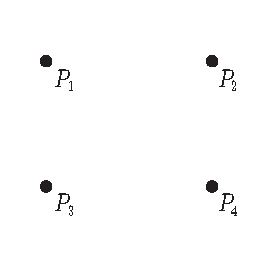
\includegraphics[trim=0cm 0cm 0cm 0cm,clip,scale=0.50]{images/fourpoints1.pdf}
\end{center}
		\item 3 punti allineati su una retta.
\begin{center}
			
\includegraphics[trim=0cm 0cm 0cm 0cm,clip,scale=0.50]{images/fourpoints2.pdf}
\end{center}
		\item 4 punti allineati su una retta.
\begin{center}
			
\includegraphics[trim=0cm 0cm 0cm 0cm,clip,scale=0.50]{images/fourpoints3.pdf}
\end{center}
	\end{itemize}
	Se i punti $P_i$ sono proiettivamente equivalenti ai punti $Q_i$, allora tali posizioni \textit{devono essere mantenute}: le proiettività mandano \textit{rette in rette}, \textit{posizioni generali in posizioni generali}. Per contronominale, se si verificano casi diversi per le due quaterne possiamo affermare che \textit{non} sono proiettivamente equivalenti.
	\begin{enumerate}
		\item Sia $P_i$, sia $Q_i$ sono in \textit{posizione generale}. Siccome abbiamo 4 punti e $4=\dim\proj[2]{\kamp}+2$, allora $\exists !$ proiettività $f$ di $\proj[2]{\kamp}$ tale che $f(P_1)=Q_i, i=1,\ \ldots,\ 4$, dunque hanno lo stesso \textit{birapporto} e sono sempre \textit{proiettivamente equivalenti}.
		\item $P_1,\ P_2,\ P_3$ \textbf{allineati ma non} $P_4$, \textbf{e lo stesso per i} $Q_i$; in altre parole, $P_1,\ P_2,\ P_3\in r$ retta proiettiva e $Q_1,\ Q_2,\ Q_3\in s$ retta proiettiva.
		\begin{center}
		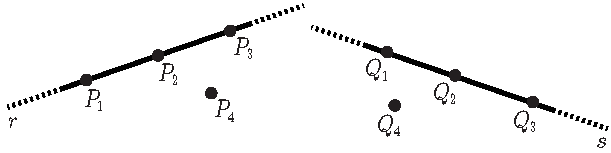
\includegraphics[trim=0cm 0cm 0cm 0cm,clip,scale=0.50]{images/fourpointseq1.pdf}
		\end{center}
		Vogliamo dimostrare che anche in questo caso le quaterne sono proiettivamente equivalenti, estendendo la proiettività fra i tre punti  al quarto.\\
		Scegliamo dei rappresentanti $P_i=[v_i],\ i=1,\ 2,\ 3,\ 4, v_i\in\kamp^3$ tale che $v_3=v_1+v_2$, lecito in quando i punti non sono allineati. Si ha che $\{v_1,\ v_2,\ v_4\}$ è una base di $\kamp^3$: $P_4\notin r$ significa che $v_4$ non è linearmente dipendente da $v_1,\ v_2$. Allo stesso modo sia $Q_i=[w_i],\ i=1,\ 2,\ 3,\ 4, w_i\in\kamp^3$ tale che $w_3=w_1+w_2$ con $\{w_1,\ w_2,\ w_4\}$ base di $\kamp^3$. Definiamo $\funz \phi {\kamp^3} {\kamp^3}$ lineare tale che:
		\begin{equation*}
			\phi(v_1)=w_1,\ \phi(v_2)=w_2,\ \phi(v_4)=w_4
		\end{equation*}
		Allora $\phi(v_3)=\phi(v_1+v_2)=w_1+w_2=w_3$ e dunque $\! \funz {f=\widetilde{\phi}} {\proj[2]{\kamp}} {\proj[2]{\kamp}}$ è una proiettività che manda $P_i$ in $Q_i,\ \forall i=1,\ 2,\ 3,\ 4$.
		\item \textbf{Tutti i punti sono allineati}.
		\begin{center}
		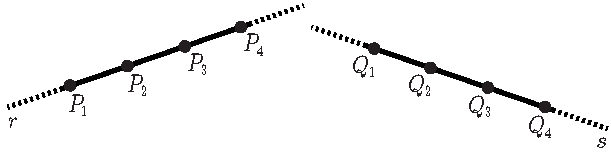
\includegraphics[trim=0cm 0cm 0cm 0cm,clip,scale=0.50]{images/fourpointseq2.pdf}
		\end{center}
		Essendo allineati, allora è definito il loro birapporto. Se le due quaterne sono proiettivamente equivalenti, sia $\funz f {\proj[2]{\kamp}} {\proj[2]{\kamp}}$ la proiettività: essa porta una quaterna nell'altra e necessariamente una retta nell'altra, ovvero $f(r)=s$; in altre parole, la restrizione alle due rette $\funz {f_{\mid_r}} r s$ porta $P_i$ in $Q_i,\ \forall i \implies \beta(P_i)=\beta(Q_i)$.\\
		Viceversa, se $\beta(P_i)=\beta(Q_i)$ allora $\exists \funz g r s$ trasformazione proiettiva che manda $P_i$ in $Q_i,\ \forall i=1,\ 2,\ 3,\ 4$.\\
		Si ha che $g$ si estende in maniera non unica ad una proiettività di $\proj[2]{\kamp}$. Infatti, dati:
		\begin{itemize}
			\item $r=\proj{U},\ U\subset \kamp^3$.
			\item $s=\proj{W},\ W\subset\kamp^3$.
		\end{itemize}
		Con $U$ e $W$ piani vettoriali, si ha che $g=\widetilde{\psi}$ con $\funz \psi U W$ è un isomorfismo lineare. Vogliamo estenderla ad un \textit{automorfismo lineare} $\funz \phi {\kamp^3} {\kamp^3}$ scegliendo basi con due vettori nel piano ed uno esterno, ovvero $u_1,\ u_2\in U$ base di $U$ e $u_3\notin U$. Dunque $\{\psi(u_1),\psi(u_2)\}$ è una base di $W$ e $w_3\notin W \implies \{u_1,u_2,u_3\}$ base di $\kamp^3$ e $\{\psi(u_1),\psi(u_2),\psi(u_3)\}$ un'altra base. Ponendo $\funz \phi {\kamp^3} {\kamp^3}$ tale che:
		\begin{itemize}
			\item $\phi(u_1)\coloneqq \psi(u_1)$.
			\item $\phi(u_2)\coloneqq \psi(u_2)$.
			\item $\phi(u_3)\coloneqq w_3$
		\end{itemize}
		Si ha $f=\widetilde{\phi}$. Dunque, i punti sono \textit{proiettivamente equivalenti} se e solo se hanno lo \textit{stesso birapporto}.
	\end{enumerate}
\vspace{-3mm}
\end{example}
\subsection{Eserciziamoci! Birapporto}
\begin{exercise}
	Verificare che se $P_1,\ P_2,\ P_3,\ P_4$ sono tutti diversi da $(1\colon 0)$, cioè $P_i=(w_i\colon 1),\ \forall i=1,\ \ldots,\ 4$ allora vale:
	\begin{equation}
		\beta=\frac{ (w_2-w_1)(w_3-w_2) }{ (w_4-w_2)(w_3-w_1) }
	\end{equation}
\vspace{-3mm}
\end{exercise}
\begin{solution}
	... %aggiungere soluzione
\end{solution}
		\section{Piano proiettivo duale}
Una \textbf{retta} in $\proj[2]{\kamp}$ ha equazione:
\begin{equation}
	r\ \colon a_0x_0+a_1x_1+a_2x_2=0
\end{equation}
Essa è un'\textbf{equazione lineare omogenea} in coordinate omogenee, dunque è determinata dai coefficienti $a_0,\ a_1,\ a_2$ dell'equazione con la proprietà che devono essere \textit{non tutti nulli}; inoltre, fissati i coefficienti, l'equazione è determinata \textit{a meno di costante moltiplicativa non nulla}. Dunque si può associare a $r$ un \textbf{punto} del piano proiettivo dato dai coefficienti delle coordinate omogenee:
\begin{equation}
	(a_0\colon a_1\colon a_2)\in\proj[2]{\kamp}
\end{equation}
Si ha una \textit{corrispondenza biunivoca} fra le rette in $\proj[2]{\kamp}$ e $\proj[2]{\kamp}$:
	% https://q.uiver.app/?q=WzAsNCxbMCwwLCJcXHtcXHRleHR7cmV0dGUgaW4gfSBcXHByb2pbMl17XFxrYW1wfVxcfSJdLFszLDAsIlxccHJvalsyXXtcXGthbXB9Il0sWzAsMSwiclxcY29sb24gYV8weF8wK2FfMXhfMSthXzJ4XzI9MCJdLFszLDEsIihhXzBcXGNvbG9uIGFfMVxcY29sb24gYV8yKSJdLFswLDEsIiIsMCx7InN0eWxlIjp7InRhaWwiOnsibmFtZSI6ImFycm93aGVhZCJ9fX1dLFsyLDMsIiIsMCx7InN0eWxlIjp7InRhaWwiOnsibmFtZSI6ImFycm93aGVhZCJ9fX1dXQ==
	\[\begin{tikzcd}
		{\{\text{rette in } \proj[2]{\kamp}\}} &&& {\proj[2]{\kamp}} \\[-25pt]
		{r\colon a_0x_0+a_1x_1+a_2x_2=0} &&& {(a_0\colon a_1\colon a_2)}
		\arrow[from=1-1, to=1-4, tail reversed]
		\arrow[from=2-1, to=2-4, tail reversed]
	\end{tikzcd}\]
% Notiamo che ciò funziona bene con $\proj[2]{\kamp}$, infatti le coordinate omogenee si comportano proprio come i coefficienti dell'equazione.
\begin{example}
In $\proj[2]{\realset}$:
		\begin{equation*}
			l_i\colon x_0+x_1+2x_2=0 \longleftrightarrow (1\colon 1\colon 2)\in\proj[2]{\realset}
		\end{equation*}
	\vspace{-6mm}
\end{example}
\begin{define}[Piano proiettivo duale.]~{}\\
	Inteso $\proj[2]{\kamp}$ come lo spazio che \textit{parametrizza le rette} in $\proj[2]{\kamp}$, lo chiamiamo \textbf{piano proiettivo duale} \index{piano!proiettivo!duale} e lo denotiamo con $\proj[2]{\kamp}^{\ast}$.
\end{define}
In prima istanza, questo significa semplicemente che si interpreta un punto del \textit{piano duale} come un punto \textit{associato} ad una \textit{retta} di $\proj[2]{\kamp}$.
%collgamento co lo spazio vettoriale duale forma lineare, prima costruzione come corrispondenza
\subsection{Fascio di rette}
\begin{define}[Fascio di rette.]~{}\\
	Un \textbf{fascio di rette}\index{fascio!di rette} $\mathcal{F}$ in $\proj[2]{\kamp}$ è l'insieme delle rette di equazione:
		\begin{equation}
			\mathcal{F}\colon \lambda l_1+\mu l_2=0, \ (\lambda\colon\mu)\in\proj[1]{\kamp}
		\end{equation}
	Dove $l_1,\ l_2$ sono due rette fissate e distinte.
\end{define}
\begin{observe}
	Possiamo pensare al fascio di rette come una \textbf{collezione di rette}, le cui equazioni si ottengono come \textit{combinazione lineare} delle due rette del fascio con $\lambda,\ \mu$ come \textbf{parametri}.
\end{observe}
\begin{example}
	Consideriamo le rette $l_1\colon x_0+x_1+2x_2=0$ e $l_2\colon 3x_0-2x_1+4x_2=0$. Il fascio di rette determinato da $l_1,\ l_2$ è
		\begin{gather*}
			(\lambda+3\mu)x_0+(\lambda-2\mu)x_1+2(\lambda+2\mu)x_2=0	
		\end{gather*}
	\begin{itemize}
		\item $(\lambda\colon\mu)=(1\colon 0) \rightarrow l_1$.
		\item $(\lambda\colon\mu)=(0\colon 1) \rightarrow l_2$.
		\item $(\lambda\colon\mu)=(1\colon 1) \colon 4x_0-x_1+6x_2=0$.	
	\end{itemize}
\vspace{-3mm}
\end{example}

\begin{observe}
	Abbiamo detto che ad ogni retta corrisponde un punto del piano proiettivo duale. Il fascio $\mathcal{F}$ corrisponde, sul piano duale $\proj[2]{\kamp}^{\ast}$, alla \textbf{retta} passante per i punti corrispondenti a $l_1$ e $l_2$:
		\begin{gather*}
			l_1\colon a_0x_0+a_1x_1+a_2x_2=0 \longrightarrow (a_0\colon a_1\colon a_2)\\
			l_2\colon b_0x_0+b_1x_1+b_2x_2=0 \longrightarrow (b_0\colon b_1\colon b_2)\\
			\mathcal{F}\colon (\lambda a_0+\mu b_0)x_0+ (\lambda a_1+\mu b_1)x_1 +(\lambda a_2+\mu b_2)x_2=0 \rightarrow (\lambda a_0+\mu b_0 \colon \lambda a_1+\mu b_1 \colon \lambda a_2+\mu b_2)
		\end{gather*}
	In altri termini, $(\lambda a_0+\mu b_0 \colon \lambda a_1+\mu b_1 \colon \lambda a_2+\mu b_2)$ rappresenta la retta per i due punti duali \textit{in forma parametrica}.
\end{observe}
\begin{example}
	Prendiamo:
		\begin{gather*}
			\begin{array}{l}
				l_1 \longleftrightarrow (1\colon 1\colon 2)=Q_1\\
				l_2\colon 3x_0-2x_1+4x_2=0 \longleftrightarrow (3\colon -2\colon 4)=Q_2\\
			\end{array}
			\mathcal{F} \longleftrightarrow (\lambda+3\mu \colon \lambda-2\mu \colon 2(\lambda+2\mu))
		\end{gather*}
	Il fascio rappresenta la retta $\overline{Q_1Q_2}$ in forma \textit{parametrica}.
\end{example}
\begin{observe}
	Siccome due rette distinte nel piano si intersecano \textit{in un punto solo}, consideriamo $P\coloneqq l_1\cap l_2$. Allora:
		\begin{itemize}
			\item Ogni retta del fascio passa per $P$ perché è lì che la combinazione lineare \textit{si annulla}.
			\item $P$ è l'unico punto comune a tutte le rette del fascio $\mathcal{F}$.
			\item Viceversa, ogni retta per $P$ appartiene al fascio $\mathcal{F}$.
		\end{itemize}
	Ciò significa che $\mathcal{F}$ è la \textit{famiglia delle rette} per il punto fissato $P$, che è detto \textbf{punto base del fascio}\index{punto!base di un fascio}.
	%P PUZZA DI SOTTOSPAZIO VETT CON VETT NULLO P
\end{observe}
\begin{example}
	Consideriamo:
		\begin{gather*}
			\begin{cases}
				l_1\colon x_0+x_1+2x_2=0\\
				l_2\colon 3x_0-2x_1+4x_2=0
			\end{cases} \implies \begin{cases}
				x_0=-x_1-2x_2\\
				-3x_1-6x_2-2x_1+4x_2=0\implies -5x_1-2x_2=0
			\end{cases}\\
		\implies \begin{cases}
			x_0=4x_1\\
			x_2=-\frac{5}{2}x_1
		\end{cases}
			\end{gather*}
		Otteniamo, a meno di multipli, il punto $P=(8\colon 2\colon -5)=l_1\cap l_2$
	Tale fascio $\mathcal{F}$ corrisponde alla retta in $\left(\proj[2]{\ }\right) ^{\ast}$ per i punti $Q_1=(1\colon 1 \colon 2)$ e $Q_2=(3\colon -2\colon 4)$ che, scritta in forma \textit{parametrica}, corrisponde a $(\lambda+3\mu \colon \lambda-2\mu \colon 2(\lambda+2\mu))$. Cerchiamo ora l'equazione \textit{cartesiana} della retta $\overline{Q_1 Q_2}$ nelle coordinate $(a_0\colon a_1\colon a_2)$:
	\begin{gather*}
	\left| \begin{array}{ccc}
		a_0 & a_1 & a_2\\
		1 & 1 & 2 \\
		3 & -2 & 4 \end{array} \right| = 8a_0 + 2a_1-5a_2=0
	\end{gather*}
	Notiamo che i coefficienti della retta ottenuta sono esattamente le \textbf{coordinate omogenee} di $P$, intersezione delle due rette!
\end{example}
Più in generale, fissato un punto base $P\in\proj[2]{\kamp}$, l'insieme delle rette per $P$ in $\proj[2]{\kamp}$:
\begin{equation}
	\mathcal{F}_P=\{\text{rette per }P\text{ in }\proj[2]{\kamp}\}
\end{equation}
È un fascio di rette corrispondente a una \textbf{retta} nel piano proiettivo duale $\left(\proj[2]{\kamp}\right)^{\ast}$. Se le coordinate del punto sono $P=(c_0\colon c_1\colon c_2)$, la retta corrispondente nel piano proiettivo duale $\left(\proj[2]{\kamp}\right)^{\ast}$ ha equazione cartesiana:
\begin{equation}
	c_0a_0+c_1a_1+c_2a_2=0
\end{equation}
Infatti, data una retta $r$ qualsiasi di equazione $a_0x_0+a_1x_1+a_2x_2=0$, il punto $P$ appartiene a $r$, cioè $P\in r$, se e solo se vale l'equazione precedente $c_0a_0+c_1a_1+c_2a_2=0$.\\
Per scrivere il fascio $\mathcal{F}$ in forma \textit{parametrica} scelgo due rette distinte passanti per $P$.
%    sostituisco le coordinate di P e trovo quell'eq:   condizione perchè appartenga alla retta   o al fascio, collezione delle rette per p     fisso p e retta che varia (duale )   retta r fissata e p che varia. Ma l'eq è la stessa. Di fatto il fascio si scrive in forma parametrica scegliendo due rette specifiche che passano per p
\begin{observe}\textsc{Interpretazione affine del fascio di rette proiettive.}\\
	Se interpretiamo $\aff{\kamp^2}=U_0\subset\proj[2]{\kamp}$ e consideriamo il fascio di rette proiettive $\mathcal{F}$ con punto base $P$ in $\proj[2]{\kamp}$, abbiamo due possibilità: $P$ è punto base \textit{proprio} o \textit{all'infinito}.
	\begin{itemize}
	\item Se $P$ è un \textbf{punto proprio}, allora $P\in\aff{\kamp^2}$ e $\mathcal{F}$ corrisponde al  \textit{rette affini} in $\kamp^2$ per il punto $P$ (passando dalla chiusura proiettiva della retta proiettiva a quella affine).
	\item Se $P$ invece è un \textit{punto improprio}, esso corrisponde ad una \textit{direzione} di rette nel piano affine e $\mathcal{F}$ corrisponde a tutte le rette affini che hanno questa direzione fissata, ovvero è un \textbf{fascio di rette parallele}.
	\end{itemize}
	Il caso proiettivo è interessante perché la distinzione fra questi due tipi di fasci è data solo dal fatto se il punto $P$ è proprio o improprio.  	
\end{observe}
\subsection{Spazi vettoriali duali e spazi proiettivi duali}
Sappiamo che $\proj[2]{\kamp}$ è il proiettivizzato di $\kamp^3$, ovvero $\proj[2]{\ }=\proj[2]{\kamp^3}$. Inoltre, in \textit{Geometria Uno}, abbiamo definito gli \textbf{spazi vettoriali duali} come\footnote{A differenza della notazione vista in \textit{Geometria Uno}, qui consideriamo gli indici delle coordinate da $0$ a $2$.}:
\begin{equation}
	\begin{array}{lll}
		\left(\kamp^3\right)^{\ast}&=&\{\text{forme lineari }\alpha\text{ su }\kamp^3\}\\
		& & \funz \alpha {\kamp^3} \kamp\\
		& & \ \, \, \alpha(x_0,\ x_1,\ x_2)= ax_0+a_1x_1+a_2x_2
	\end{array}
\end{equation}
Quando consideriamo la retta $r\colon a_0x_0+a_1x_1+a_2x_2=0$, $r$ è il proiettivizzato del \textbf{nucleo} di $\alpha$, il quale è un \textit{piano vettoriale} $\ker\alpha\subset\kamp^3$ la cui equazione è appunto $a_0x_0+a_1x_1+a_2x_2=0$.\\
In altre parole, si ha una corrispondenza fra i \textit{punti della retta proiettiva duale} e le \textit{classi proiettive} delle forme lineari $[\alpha]$:
\begin{equation}
	\begin{array}{ccc}
		\left( \proj[2]{\ }\right)^{\ast}&=&\proj[2]{\kamp^3}^{\ast}\\
		r & \longleftrightarrow & [\alpha]\\
	\end{array}
\end{equation}
Infatti, $\alpha$ è una forma lineare \textit{non nulla} determinata \textit{a meno di multipli}. Si ha che $\{x_0,\ x_1,\ x_2\}$ è una base di $(\kamp^3)^{\ast}$ che induce le coordinate proiettive $(a_0\colon a_1\colon a_2)$ su $\left( \proj[2]{\ }\right)^{\ast}$.\\
Pertanto, tale \textit{interpretazione astratta} diventa operativa fissando la \textit{base duale} delle forme lineari: scrivo $\alpha$ come combinazione lineare della base, e i coefficienti saranno le  data dalle \textit{coordinate proiettive associate}.
Generalizziamo ulteriormente ad uno spazio vettoriale qualunque.
\begin{define}[Spazio proiettivo duale.]~{}\\
	Dato uno spazio vettoriale $V$, il suo \textit{spazio proiettivo associato} $\proj{V}$ ed il suo \textit{spazio vettoriale duale} $V^{\ast}=\{\text{forme lineari }\funz \alpha V \kamp \}$, si definisce lo \textbf{spazio proiettivo duale}\index{spazio!proiettivo!duale} di $\proj[n]{V}$:
	\begin{equation}
		\proj{V}^{\ast}=\proj{V^{\ast}}
	\end{equation}
	Poiché $\dim V^{\ast} = \dim V$, allora $\proj{V}^{\ast} =\proj{V}$.
\end{define}
In particolare, si ha la corrispondenza biunivoca:
% https://q.uiver.app/?q=WzAsNCxbMCwwLCJcXHByb2p7Vn1ee1xcYXN0fSJdLFszLDAsIlxce1xcdGV4dHtpcGVycGlhbmkgZGkgfSBcXHByb2p7Vn0gXFx9Il0sWzAsMSwiW1xcYWxwaGFdIl0sWzMsMSwiXFxwcm9qe1xca2VyXFxhbHBoYX1cXHN1YnNldFxcbWF0aGJie1B9KFYpIl0sWzAsMSwiIiwwLHsic3R5bGUiOnsidGFpbCI6eyJuYW1lIjoiYXJyb3doZWFkIn19fV0sWzIsMywiIiwwLHsic3R5bGUiOnsidGFpbCI6eyJuYW1lIjoiYXJyb3doZWFkIn19fV1d
\[\begin{tikzcd}
	{\proj{V}^{\ast}} &&& {\{\text{iperpiani di } \proj{V} \}} \\
	{[\alpha]} &&& {\mathbb{P}\left(\ker \alpha\right)\subset\proj{V}}
	\arrow[from=1-1, to=1-4, tail reversed]
	\arrow[from=2-1, to=2-4, tail reversed]
\end{tikzcd}\]
In coordinate, ad un piano di equazione $a_0x_0+\ldots +a_nx_n=0$ associamo il punto $(a_0\colon\ldots\colon a_n)$, nello stesso modo in cui ad un vettore associo i coefficienti della scrittura secondo una tale base.
\subsection{Impratichiamoci! Piano proiettivo duale}
\begin{exercise}
	In $\proj[2]{\realset}$ scrivere in forma parametrica il fascio delle rette per il punto base $P$ di coordinate $(1\colon -1 \colon 4)$.
\end{exercise}
\begin{solution}
	Scegliamo 2 rette distinte, a nostro piacere, che passano per il punto $P$; ad esempio, $l_1\colon x_0+x_1=0$ e $l_2\colon 4x_0-x_2=0$. Il fascio sarà:
	\begin{gather*}
		\begin{array}{cc}
			\mathcal{F}\colon \lambda(x_0+x_1)+\mu(4x_0-x_2)=0 &  \\
			(\lambda+4\mu)x_0+\lambda x_1-\mu x_2=0,\ & (\lambda\colon\mu)\in\proj[1]{\ }
		\end{array}
	\end{gather*}
	Se facciamo variare $\lambda$ e $\mu$ otteniamo tutte le rette di $\proj[2]{\realset}$ che passano per $P$.
\end{solution}
